\documentclass{scrartcl}

%This template is based on the DFG rtf form (see Readme on GitHub for last accessed date, and version in the header of the compiled PDF)
%
%Author: Martin Hoelzer, hoelzer.martin@gmail.com
%

\usepackage[utf8]{inputenc}
\usepackage[english]{proposal}
\usepackage{subcaption}
\newcommand{\sg}[1]{{\color{red}#1}}
\newcommand{\mr}[1]{{\color{blue}#1}}

% final version?
\setboolean{finalcompile}{false}

% show DFG template version the current LaTeX template is based on in the header. Will be deactivated when 'finalcompile' is set 'true'
\ifthenelse{\boolean{finalcompile}}{}{\ihead*{DFG-form 53.01 - 03/25}}

% all config is done in Header.tex
\ifthenelse{\boolean{finalcompile}}{
  \usepackage[disable]{todonotes}
  \usepackage[final]{showlabels}
}{
  \usepackage{todonotes}
  %\setlength{\marginparwidth}{2cm}
  \paperwidth=\dimexpr \paperwidth + 6cm\relax
  \oddsidemargin=\dimexpr\oddsidemargin + 3cm\relax
  \evensidemargin=\dimexpr\evensidemargin + 3cm\relax
  \marginparwidth=\dimexpr \marginparwidth + 3cm\relax
  \usepackage{showlabels}
}

\usepackage{amssymb}
\usepackage{lipsum}
\usepackage[pdftex, colorlinks=true, linkcolor=MidnightBlue, citecolor=MidnightBlue, urlcolor=MidnightBlue, pdfauthor={Dr.\ Martin Hoelzer}, pdfpagelayout=SinglePage, bookmarks, bookmarksopen]{hyperref}

\usepackage{gensymb}
\usepackage{graphicx}
\usepackage{wrapfig}
\usepackage{booktabs}

\usepackage{textcomp}
\usepackage{mathtools}
\usepackage{relsize}
\usepackage{tikz}
\usetikzlibrary{arrows.meta}

% Fix font warnings for verbatim braces
\DeclareTextSymbolDefault{\textbraceleft}{T1}
\DeclareTextSymbolDefault{\textbraceright}{T1}

\usepackage[numbered]{bookmark}

%\usepackage{titlesec}
%\usepackage{placeins}

\usepackage[font=small,labelfont={bf,it},textfont=it]{caption}
\captionsetup{format=plain}

\usepackage[noabbrev,capitalise]{cleveref}
% see also: https://www.namsu.de/Extra/pakete/Cleveref.html

% make numbers look better in funding section
%siunitx package is loaded already in proposal.sty
\sisetup{detect-all=true}

\graphicspath{{figures/}}

% command \todo now deprecated by using todonotes
%\newcommand{\todo}[1]{\xspace{\textcolor{red}{\bfseries[TODO: #1]}}\xspace}
\newcommand{\cp}[1]{\xspace{\textcolor{blue}{\bfseries[COPIED: #1]}}\xspace}
\renewcommand{\todo}[1]{\xspace{\textcolor{red}{\bfseries[TODO: #1]}}\xspace}

\input{highlight_box.tex}

% "Klemmer et al., incl. Rußwurm (2025)"
\newcommand{\citepPIRusswurm}[2][]{%
  \citeauthor{#2}, incl.\ Ru\ss{}wurm\ (\citeyear[#1]{#2})%
}

% textual variant: "Klemmer et al., incl. Rußwurm (2025) show ..."
\newcommand{\citetPIRusswurm}[2][]{%
  \citeauthor{#2}, incl.\ Ru\ss{}wurm\ (\citeyear[#1]{#2})%
}

% "Klemmer et al., incl. Garaba (2025)"
\newcommand{\citepPIGaraba}[2][]{%
  \citeauthor{#2}, incl.\ Garaba\ (\citeyear[#1]{#2})%
}

% Preamble
\usepackage[most]{tcolorbox}
\usepackage{wrapfig}
\usepackage{xcolor}

% A reusable WP side-box
\newcommand{\WPsidebox}[3]{%
\begin{wrapfigure}[#3]{r}{0.43\textwidth}
\vspace{-0.8\baselineskip} % tweak if needed
\begin{tcolorbox}[
  enhanced,
  colback=gray!3,
  colframe=gray!60,
  boxrule=0.6pt,
  arc=2mm,
  left=1.5mm,right=1.5mm,top=1.2mm,bottom=1.2mm,
  fonttitle=\bfseries,
  title=#1,
]
\footnotesize
#2
\end{tcolorbox}
\vspace{-0.8\baselineskip} % tweak if needed
\end{wrapfigure}%
}


% language dependent
% change labels, e.g.:
\setkomafont{paragraph}{\normalfont\itshape}


%%%%%%%%%%%%%%%%%%%%%%%%%%%%%%%%%%%%%%%%%%%%%%%%%%%%%%%%%%%%%%%%%%%%%%%%%%%%%
%%%%  TITLE PAGE  %%%%%%%%%%%%%%%%%%%%%%%%%%%%%%%%%%%%%%%%%%%%%%%%%%%%%%%%%%%
%%%%%%%%%%%%%%%%%%%%%%%%%%%%%%%%%%%%%%%%%%%%%%%%%%%%%%%%%%%%%%%%%%%%%%%%%%%%%

\newcommand{\applicants}{Marc Rußwurm, Rheinische Friedrich-Wilhelms-Universität Bonn
 (UoB) \\ Shungudzemwoyo Garaba, Carl von Ossietzky Universität Oldenburg (UOL)}
\newcommand{\project}{STREAM: Spectral and Geospatial Inference for Riverine Plastic Monitoring}

% add bib entries here that you want to highlight in the text and publication list (bold)
% \addtocategory{important}{}

\begin{document}
\pagestyle{empty}
\setcounter{page}{1}

%%%%%%%%%%%%%%%%%%%%%%%%%%%%%%%%%%%%%%%%%%%%%%%%%%%%%%%%%%%%%%%%%%%%%%%%%%%%%%
%% A NICE TITLE PAGE - OPTIONAL BC NOT IN THE ORIGINAL DFG TEMPLATE
% if you use the title page, set the \setcounter{page}{0} above!
%%%%%%%%%%%%%%%%%%%%%%%%%%%%%%%%%%%%%%%%%%%%%%%%%%%%%%%%%%%%%%%%%%%%%%%%%%%%%%
% {\selectlanguage{english}

  \vspace*{20ex}

  \begin{center}
  \large

  {\bfseries Proposal to the Deutsche Forschungsgemeinschaft\\(German Research Foundation)}

  Kennedyallee 40, 53175 Bonn

  \vspace{4ex}

  on the granting of a research project

  \vspace{9ex}

  \begin{bfseries}
    This is a fancy project title to rule the world
  \end{bfseries}

  \medskip

	\todo{First-time} Research Grant

  \vspace{9ex}

	\vspace{9ex}

	\today
  \end{center}
}


%%%%%%%%%%%%%%%%%%%%%%%%%%%%%%%%%%%%%%%%%%%%%%%%%%%%%%%%%%%%%%%%%%%%%%%%%%%%%
%%%%  MAIN MATTER  %%%%%%%%%%%%%%%%%%%%%%%%%%%%%%%%%%%%%%%%%%%%%%%%%%%%%%%%%%
%%%%%%%%%%%%%%%%%%%%%%%%%%%%%%%%%%%%%%%%%%%%%%%%%%%%%%%%%%%%%%%%%%%%%%%%%%%%%
\cleardoublepage
\pagestyle{plain}

%%%%%%%%%%%%%%%%%%%%%%%%%%%%%%%%%%%%%%%%%%%%%%%%%%%%%%%%%%%%%%%%%%%%%%%%%%%%%
%%%% For first-time proposals, please also note the following: Please provide a
% concise description of your previous postgraduate training and research,
% highlighting your abilities and demonstrating that you are capable of carrying
% out the proposed project. Describe your scientific track record to date,
% mentioning research topics that you've worked on so far. Previous scientific
% accomplishments must not be directly related to the project.

%%%%%%%%%%%%%%%%%%%%%%%%%%%%%%%%%%%%%%%%%%%%%%%%%%%%%%%%%%%%%%%%%%%%%%%%%%%%%%%
%%%%  PROJECT DESCRIPTION - PROJECT PROPOSALS  %%%%%%%%%%%%%%%%%%%%%%%%%%%%%%%%
%%%%%%%%%%%%%%%%%%%%%%%%%%%%%%%%%%%%%%%%%%%%%%%%%%%%%%%%%%%%%%%%%%%%%%%%%%%%%%%
%% Sections 1-3 must not exceed 17 pages in total.
{\raggedright{} \normalsize \bfseries 
	Project Description -- Project Proposals \newline \par
	\applicants{} \newline \par
	\project{} \par
	\rule{\textwidth}{0.5pt} \par
	%Project Description
}


%%%%%%%%%%%%%%%%%%%%%%%%%%%%%%%%%%%%%%%%%%%%%%%%%%%%%%%%%%%%%%%%%%%%%%%%%%%%%
%%%%  STATE OF THE ART AND PRELIMINARY WORK %%%%%%%%%%%%%%%%%%%%%%%%%%%%%%%%%
%%%%%%%%%%%%%%%%%%%%%%%%%%%%%%%%%%%%%%%%%%%%%%%%%%%%%%%%%%%%%%%%%%%%%%%%%%%%%
\section{Starting Point}
\label{sec:work-report}

Despite decades of awareness and policy activity, society still lacks reliable, comparable, and uncertainty-quantified estimates of how much \emph{floating macrolitter} is transported by major European rivers \citep{gonzalez2021floating,weiss2021missing,oswald2026}. Even for the river Rhine, one of the best-instrumented river systems in Europe, recent studies report strikingly different transport estimates and point to substantial \emph{unaccounted-for litter}: a 16-month interception study near Cologne estimates an annual macrolitter transport of roughly \(\sim\)3{,}000--4{,}700\,tonnes per year (tpy) towards the North Sea \citep{gnann2026river}, whereas downstream observational estimates for floating plastic transport in the Rhine--Meuse delta near Rotterdam are far lower, on the order of \(\sim\)65\,tpy, with strong variability driven by hydrology \citep{van2022hydrology}. This difference is not presented here as a simple contradiction, since real downstream processes such as retention, temporary storage, vertical mixing, fragmentation, and redistribution may explain part of the gap. However, its magnitude makes clear that current monitoring practice is not yet sufficiently harmonized to disentangle physical loss processes from methodological differences across sites, time periods, and sensing approaches \citep{Gallitelli2024,smith2025insights,oswald2026}.

This bottleneck is not solved automatically by the increasing availability of sensing technologies such as continuous RGB camera streams, UAV surveys, airborne spectroscopy, and high-revisit satellite imagery. On the contrary, the rapid growth in multi-source imagery shifts the main challenge from data acquisition to \emph{data integration and inference}. Different sensing modalities observe different aspects of the river system, at different spatial and temporal scales, with different error structures and under different environmental conditions. As a consequence, the key scientific challenge is no longer only to detect litter somewhere in the river corridor, but to infer comparable and uncertainty-aware indicators of litter occurrence, concentration, and ultimately transport from heterogeneous observations. In other words, local detections, spectral anomalies, and physical interception data must be translated into a common probabilistic representation of riverine litter dynamics. Addressing the Rhine discrepancy therefore requires not only better sensing, but methodological foundations for harmonizing multimodal observations and integrating them into a consistent monitoring framework with explicit uncertainty propagation.

This challenge is scientifically important because rivers are widely recognized as major pathways transporting mismanaged plastic waste from land into aquatic and marine environments \citep{caspers1987gesamp,unep2021,galgani2024revisiting}. Global synthesis studies estimate that rivers deliver on the order of \(\sim\)1--3\,million tonnes of plastic per year to the ocean, with emissions concentrated in a subset of river systems \citep{lebreton2017river,meijer2021more}. At the same time, scenario studies suggest that without effective mitigation, annual plastic emissions to aquatic systems may continue to grow substantially over the coming decades \citep{pew2020breaking,unsecretariat2025worldenvironmentday,deeney2026global}. Translating these global narratives into actionable mitigation, however, requires sustained and spatially resolved river-basin observations with explicit uncertainty quantification---precisely where existing monitoring practice remains weakest.

The Rhine basin is an ideal methodological testbed for this challenge. First, it combines high societal relevance with comparatively low macrolitter loads, meaning that methods robust enough for the Rhine are likely transferable to more polluted river systems where litter signals may be easier to detect. Second, the basin already hosts complementary monitoring activities, including interception-based observations near Cologne \citep{gnann2026river} and long-duration transport studies in the Rhine--Meuse delta \citep{van2022hydrology}, thereby offering a strong empirical basis for calibration and comparison. Third, the Rhine is covered by a dense Earth-observation and environmental data ecosystem, including satellite imagery, airborne campaigns, hydrological observations, and GIS context layers. Together, these characteristics make the basin well suited not simply for another local case study, but for developing and evaluating the scientific and methodological foundations of an uncertainty-aware monitoring framework.

Existing monitoring approaches remain fragmented across spatio-temporal scales. On the ground, standard monitoring still relies heavily on manual visual counting and localized campaigns, which are labour-intensive and difficult to maintain at high temporal frequency across many sites. Bridge-mounted cameras combined with deep learning can automate detection and yield continuous time series \citep{vanlieshout2020automated}, and our own collaborative work has demonstrated object-detection pipelines under realistic river conditions and confounding backgrounds \citepPIRusswurm{hagenbeek5841770exploring}. Yet the translation from local detections to comparable transport indicators remains uncertainty-dominated \citep{vriend2025uncertainties}, motivating harmonized observation protocols \citep{vanemmerik2023harmonized} and methods that propagate uncertainty from detection to higher-level inference \citep{cottom2024local}.

From an Earth-observation perspective, remote sensing offers the possibility to extend monitoring beyond isolated field sites, but it faces two persistent challenges: limited detectability against water and complex backgrounds, and the lack of consistent ground validation across scales. Diagnostic optical properties of plastic-rich litter have been documented using spectroscopic measurements from the visible to shortwave infrared range, providing a physical basis for multi- and hyperspectral sensing \citep{garaba2018airborne,garaba2020uvswir,goddijn2018concept,garaba2021concentration,knaeps2021hyperspectral,de2023hyperspectral,giz2023}. Recent studies further show that riverine litter can be detected and quantified from very fine resolution multispectral satellite imagery when sensor properties, spatial context, and transferability constraints are carefully considered \citep{garaba2024riverine,smith2025insights}. However, no single modality provides complete or uniformly reliable evidence across all river sections and conditions. This makes riverine litter monitoring fundamentally a problem of \emph{multimodal probabilistic integration}.

Taken together, these limitations show that the central challenge is no longer merely to collect more observations, but to turn heterogeneous observations into comparable and uncertainty-aware evidence. What is needed are the scientific and methodological foundations for a monitoring framework that can integrate multimodal data across scales in a transparent and probabilistically consistent way.

\subsection*{State of the art and preliminary work}

\textbf{Bayesian Inference} provides a natural yet largely unexplored framework for riverine plastic litter monitoring because the target variables of interest are inherently uncertain, sparse, and only partially observable. Plastic presence, litter concentration, and transport are not measured directly and consistently at all locations and times, but must instead be inferred from heterogeneous evidence streams that differ in spatial support, temporal frequency, reliability, and modality. Bayesian hierarchical models are particularly well suited to such settings because they separate the latent environmental process from the observation process and propagate uncertainty through the full inference chain \citep{wikle1998hierarchical,wikle2003hierarchical}. This is especially attractive in the present project, where large-scale geospatial context can inform prior expectations about litter accumulation and transport, while spectral and visual observations provide local evidence about actual litter presence.

More broadly, Bayesian models offer three advantages for this application. First, they provide a coherent mechanism for integrating multiple modalities and scales, ranging from bridge-based cameras and UAV imagery to airborne hyperspectral data and satellite observations. Second, they explicitly quantify uncertainty, which is essential when predictions are used to guide monitoring, reporting, and intervention. Third, they allow prior knowledge to be represented transparently rather than remaining entangled in a purely discriminative predictor. Related Bayesian fusion approaches have already proven useful in environmental and remote-sensing applications, including spatiotemporal image fusion, the integration of in situ and satellite observations, and hierarchical space-time modeling \citep{xue2017bayesian,chen2021novel,he2024spatiotemporal}. The novelty of the present proposal is therefore not Bayesian inference per se, but its use as a unified framework to decompose riverine litter monitoring into environmental priors, observation likelihoods, and uncertainty-aware posterior estimates that are comparable across sensing modalities.

Conceptually, the proposed framework is related to \emph{product-of-experts} formulations, in which multiple sources of evidence are combined multiplicatively to constrain the posterior distribution \citep{hinton1999temporal}. In the context of this proposal, geospatial embeddings act as one expert by providing environmental priors over locations, while spectral and image-based observations act as complementary experts that contribute likelihood terms. Although multimodal fusion is common in environmental monitoring and machine learning, such a systematic Bayesian decomposition into environmental priors and observational likelihoods has, to our knowledge, not yet been investigated for riverine plastic litter monitoring in a unified and uncertainty-aware framework.

\begin{figure}
    \centering
    \begin{subfigure}{0.49\textwidth}
        \centering
        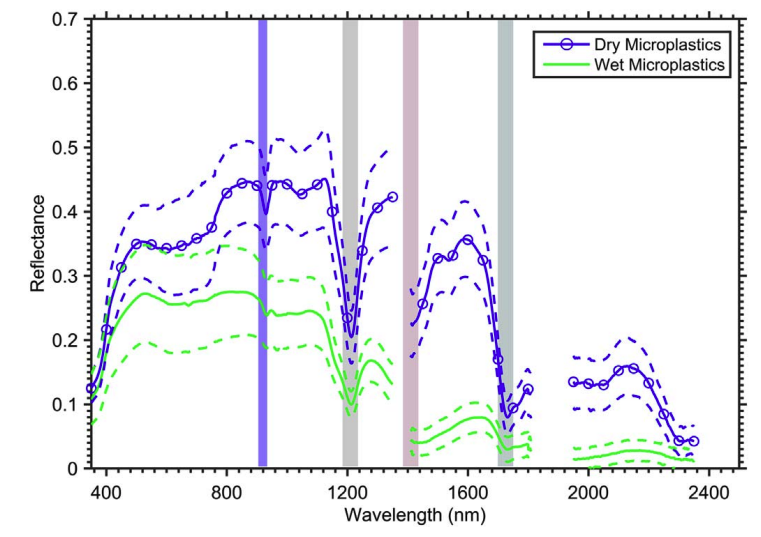
\includegraphics[width=\textwidth]{figures/garaba_spectra.png}
        \caption{Remote sensing spectra provide the \textbf{likelihood of plastic presence}, here illustrated by lab spectra from dry and wet microplastics by \citep{garaba2018airborne}.}
        \label{fig:spectra}
    \end{subfigure}
    \hfill
    \begin{subfigure}{.5\textwidth}
        \centering
        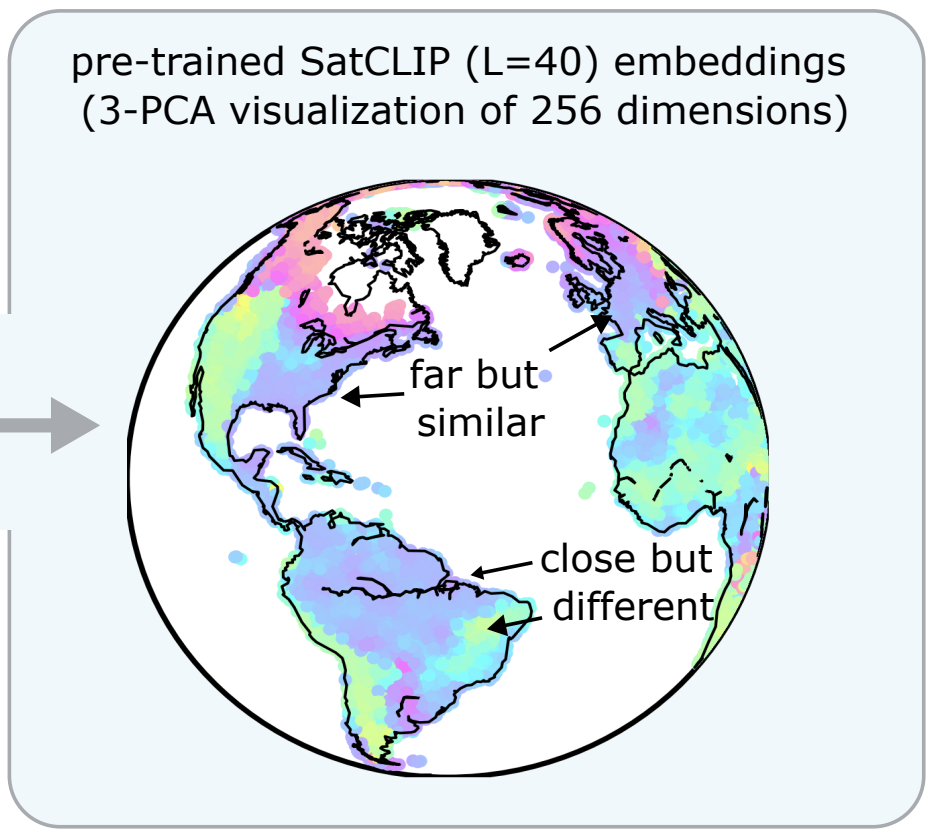
\includegraphics[width=.75\textwidth]{figures/satclip.png}
        \caption{Spatial embeddings can serve as \textbf{environmental priors}, where nearby locations can be dissimilar in semantic embedding space \citepPIRusswurm{klemmer2025satclip}.}
        \label{fig:satclip}
    \end{subfigure}
    \caption{Complementary expertises of PIs Garaba and Ru{\ss}wurm within the proposed Bayesian framework. Spatial embeddings (core expertise PI Ru{\ss}wurm) provide continuous large-scale environmental priors that support the analysis of litter reflectances (core expertise PI Garaba) as observational likelihoods of plastic presence.}
    \label{fig:coreexpertise}
\end{figure}

\textbf{Geospatial Priors through Implicit Neural Representations (Core Expertise PI Ru{\ss}wurm)} Recent work in geospatial machine learning has shown that neural networks can learn location-dependent prior information directly from coordinates and associated environmental data. Such \emph{location encoders} or \emph{geopriors} provide a continuous alternative to discretized spatial gridding and enable probability estimates to be associated with arbitrary locations \citep{russwurm2024geographic,mac2019presence,cole2023spatial}. This paradigm has proven particularly effective in ecological prediction and species distribution modeling, where spatial context strongly shapes the plausibility of observations. In the context of riverine litter, comparable location-dependent priors are attractive because litter occurrence and transport are also shaped by spatially structured environmental factors such as river morphology, adjacent land use, urbanization, hydrological regime, floodplain structure, and likely retention or accumulation zones. Beyond scalar prior prediction, current research increasingly aims to learn rich geospatial representations in the form of semantically meaningful embeddings. These embeddings can be trained in a self-supervised manner from large multimodal Earth observation archives and encode similarities between places that go beyond geographic proximity alone \citepPIRusswurm{klemmer2025earth,klemmer2025satclip}. As illustrated by SatCLIP in \cref{fig:satclip}, geographically distant regions may be similar in embedding space because they share environmental structure, while nearby locations may differ strongly due to land cover, hydrology, or human activity. Such embedding spaces are therefore highly attractive as environmental priors for plastic litter monitoring, since they allow the transfer of evidence across environmentally similar river sections rather than relying only on Euclidean distance. Developing accurate, high-capacity, and regionally adaptive geospatial representations is currently an active research direction \citepPIRusswurm{rao2026localized}, and the present proposal builds directly on these advances.

\textbf{Spectral Analysis and Litter Likelihood (Core Expertise PI Garaba)} A central challenge in plastic litter monitoring is that plastic must be distinguished from a wide range of natural and anthropogenic materials under highly variable environmental conditions. PI Garaba has established an internationally visible research profile in hyperspectral optical remote sensing of aquatic litter, with methodological expertise spanning ultraviolet, visible, near-infrared, shortwave infrared, and thermal observations from laboratory, field, airborne, and satellite platforms \citep{garaba2018airborne,garaba2020uvswir,garaba2022toa,garaba2021concentration,garaba2024riverine,ohall6138760plastic}. His work has advanced both the physical understanding of plastic reflectance behavior and the methodological foundations for detecting floating litter under realistic environmental conditions. This includes not only the characterization of spectral signatures across sensing scales, but also broader conceptual contributions such as the \enquote{detect, identify, quantify, track} capability matrix for remote sensing of floating litter \citep{garaba2024riverine}. Hyperspectral and multispectral remote sensing provide a physically grounded route to this problem because plastics exhibit diagnostic reflectance behavior that can, in principle, be separated from surrounding water, sediment, foam, vegetation, drift material, and other floating objects. This spectral basis is illustrated in \cref{fig:spectra}, which shows representative reflectance differences between dry and wet microplastics from \citep{garaba2018airborne}. PI Garaba’s prior work has also clarified the major confounding factors that limit operational detectability, including wetness, biofouling, sub-pixel mixing, atmospheric effects, turbidity, and illumination variability \citep{garaba2018airborne,garaba2020uvswir,garaba2024riverine}.  This challenge further motivates the importance of imaging spectroscopy. Hyperspectral technologies spanning the visible to shortwave infrared range have long been recognized as highly relevant for identifying natural and anthropogenic materials across diverse environments \citep{cloutis1989spectral,kuhn2004hydrocarbon,goddijn2018concept,knaeps2021hyperspectral,de2023hyperspectral,ohall6138760plastic}. In the context of riverine plastic litter, they offer the prospect of moving beyond anomaly detection toward more specific material discrimination under complex environmental backgrounds. However, their application to riverine plastic monitoring from current spaceborne systems such as EnMAP, EMIT, or PRISMA remains largely unexplored, particularly in combination with coincident airborne surveys and in-situ sampling for validation and the expansion of spectral reference libraries. Bridging this gap is a key opportunity for the present proposal.

\textbf{Litter quantification methodologies} A key methodological challenge in riverine plastic monitoring is not only to detect litter, but to quantify it in a way that is comparable across platforms, scales, and observation protocols. Existing approaches range from direct physical sampling and manual counting to image-based detection from proximal, aerial, and satellite sensors. These methods differ substantially in what they measure, for example item counts, areal coverage, transport flux, or inferred likelihood of plastic presence, and each comes with distinct uncertainty sources. Together, they define the current methodological landscape on which the proposed framework builds.

\begin{description}
    \item[Ground data collection]
    Ground-based quantification remains the essential reference for calibration and validation because it provides the closest link to physically observed litter items, composition classes, and transport estimates. This includes labour-intensive sampling and interception approaches such as litter traps, cleanup-based quantification, and long-term deployed interception systems, which can support direct estimates of transported macrolitter and composition over time \citep{gnann2026river,martinezvicente2019measuring,vighi2022monitoring}. In river settings, bridge-based visual counting has further emerged as a practical method to estimate floating litter transport at fixed cross-sections \citep{van2022hydrology}. Recent work has shown that such workflows can be partially automated using deep-learning-based object detection from bridge-mounted cameras, including under realistic confounding conditions such as dense vegetation and water hyacinths \citep{vanlieshout2020automated,hagenbeek5841770exploring}; see also \cref{fig:plastichyacinths}. More broadly, proximal imaging has also been explored in maritime contexts, for example through container-ship-based visual litter detection at sea \citep{de2021quantifying}. Despite their high value, these ground and proximal approaches remain site-specific, labour-intensive, and sensitive to protocol choices and visibility conditions, which motivates harmonized and uncertainty-aware integration with larger-scale observations \citep{vriend2025uncertainties,vanemmerik2023harmonized,blettler2026macroplastic}.

    \item[UAV monitoring]
    Uncrewed aerial vehicles provide a flexible intermediate scale between field observations and satellite monitoring and have become an important tool for mapping floating and stranded plastic litter at high spatial resolution. UAVs are particularly useful for targeted campaigns, controlled experiments, and validation settings because they can capture fine-grained object structure while covering larger areas than ground surveys. Prior work by PI Garaba has demonstrated machine-learning-based UAV methodologies for plastic litter quantification and likelihood estimation \citepPIGaraba{wolf2020aplasticq}; see \cref{fig:preliminary_work_a}. Related studies have further shown the value of UAV and low-altitude multispectral observations for detecting and mapping litter under controlled and semi-natural conditions \citep{geraeds2019uav,cortesi2022uavmultispectral,valenzuela2026mapping,topouzelis2019detection,papageorgiou2022sentinel2}. UAV observations are therefore a critical bridge between in-situ measurements and synoptic remote sensing, but their transferability across sites, seasons, and environmental backgrounds remains limited without systematic calibration and sensor-aware modeling \citep{garaba2020uvswir,garaba2024riverine,giz2023,hu2025logic}.

    \item[Satellite monitoring of rivers and open water]
    Satellite remote sensing offers the only realistic pathway toward synoptic, repeated, and basin-scale monitoring of floating litter. In river systems, recent work has shown that plastic-related anomalies and litter hotspots can be identified from multispectral imagery such as Sentinel-2 and PlanetScope using scalable machine-learning pipelines \citepPIRusswurm{perez2025scalable}; see \cref{fig:preliminary_work_c}. For marine and open-water settings, related large-scale screening approaches have also been demonstrated from Sentinel-2 archives \citep{russwurmcell2023}. More generally, recent studies indicate that high-resolution multispectral imagery can support mapping of riverine litter patches, including from PlanetScope, Sentinel-2, and SkySat data \citep{garaba2024riverine,mohsen2023machine,smith2025insights}. These approaches provide a major step toward operational large-scale monitoring, but most current products still reflect anomaly detection or inferred litter presence rather than definitive material identification or directly comparable quantitative estimates. Their interpretation is further complicated by mixed pixels, spectral ambiguity, varying optical water conditions, domain shift across sites and seasons, and the scarcity of coincident reference data for robust validation \citep{biermann2020finding,bansal2025efficient,cerra2024detection,wang2026detecting,samuriwo2024comparative,marye2025remote}. Satellite observations are therefore powerful for large-scale screening and likelihood estimation, but they require calibration against proximal and in-situ observations and benefit strongly from integration with environmental prior information.
\end{description}

Taken together, these approaches provide complementary but non-commensurate observations of riverine litter, ranging from direct counts and transport estimates to image-based likelihoods of presence. Their differing spatial support, temporal coverage, and uncertainty characteristics are precisely what motivate the Bayesian integration framework proposed in this project.

\begin{figure}
    \centering
    \begin{subfigure}[t]{\textwidth}
        \centering
        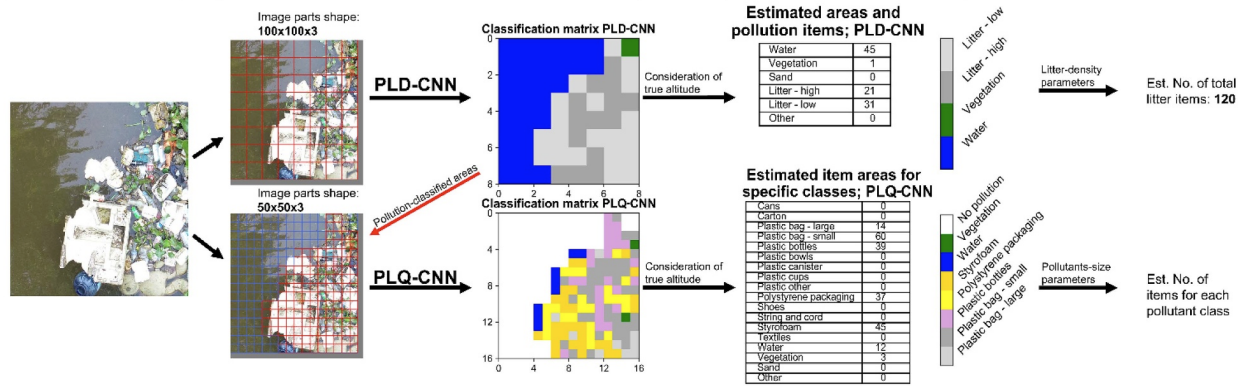
\includegraphics[width=\textwidth]{figures/wolf_garaba_et_al.png}
        \caption{Litter likelihood estimation methodology from UAV imagery by \citepPIGaraba{wolf2020aplasticq}.}
        \label{fig:preliminary_work_a}
    \end{subfigure}

    \vspace{0.5em}

    \begin{subfigure}[t]{0.395\textwidth}
        \centering
        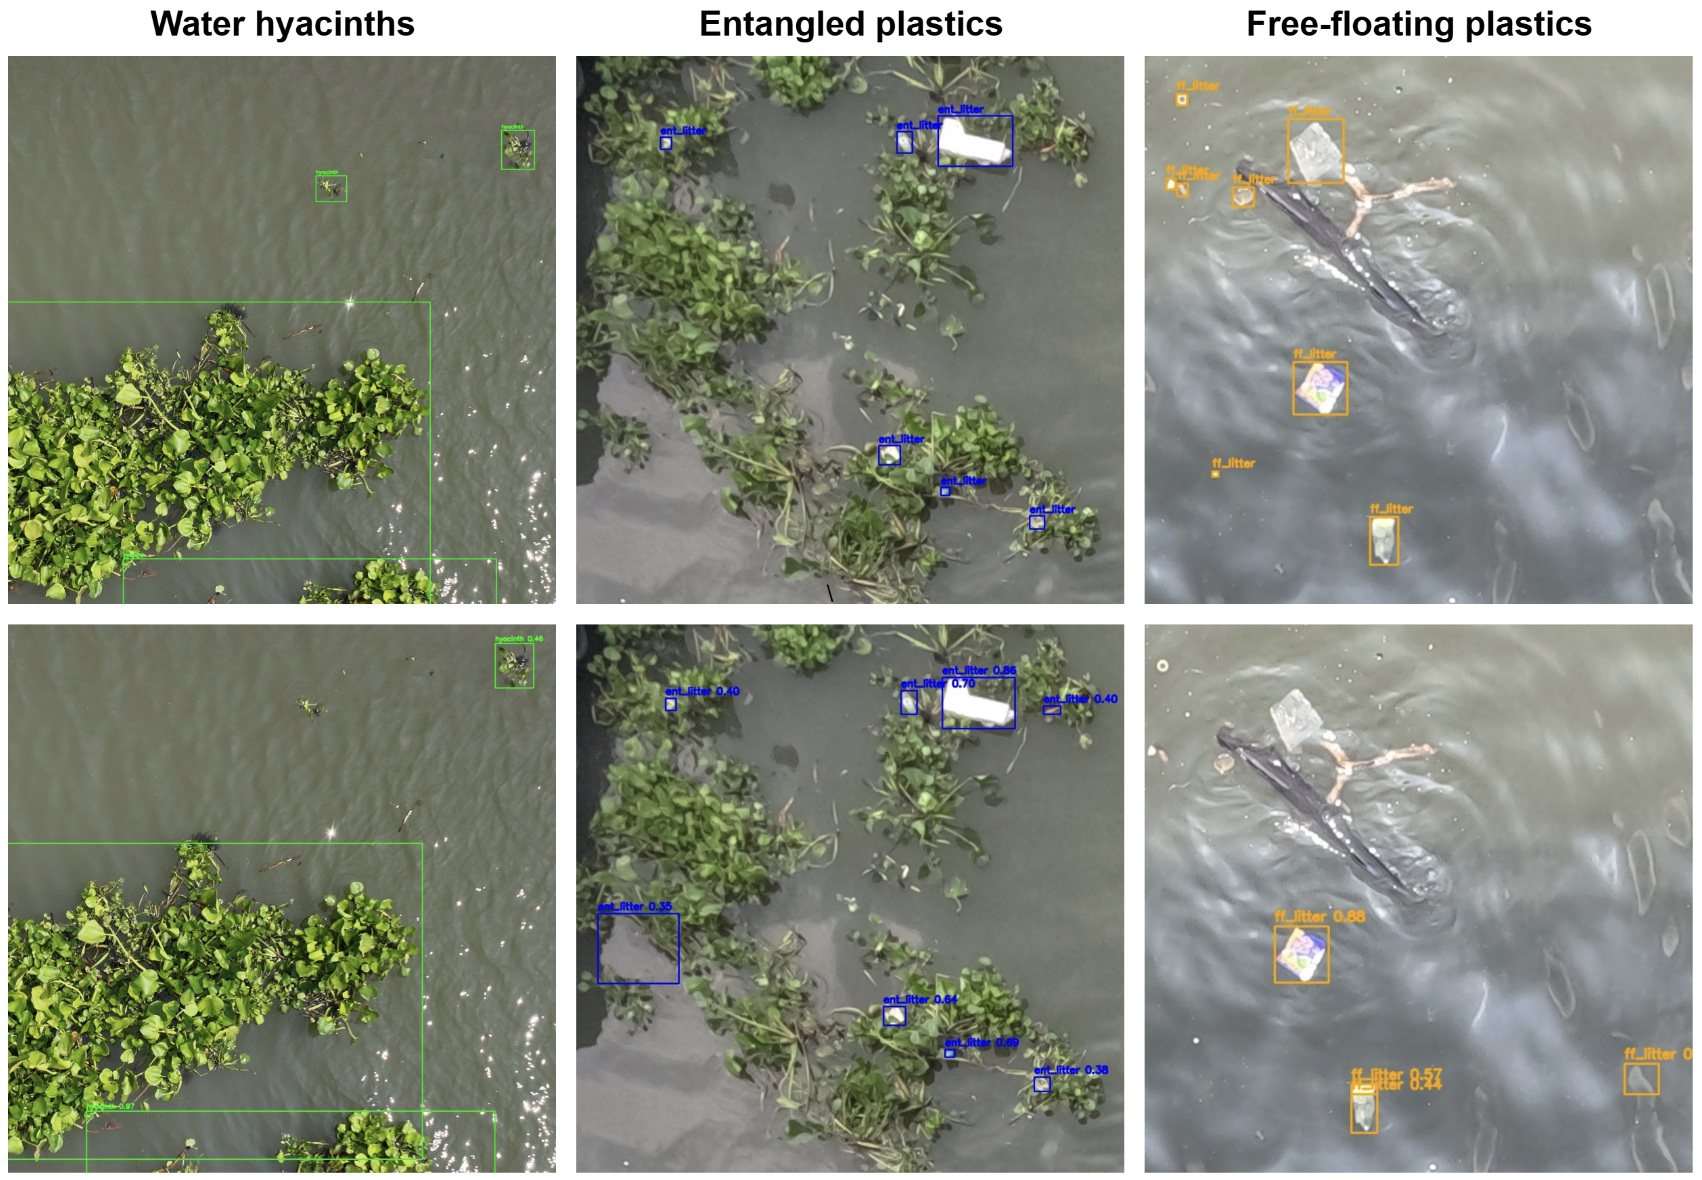
\includegraphics[width=\textwidth]{figures/Haagenbeek_bounding_boxes.png}
        \caption{Litter detection from bridges within hyacinths \citepPIRusswurm{hagenbeek5841770exploring}.}
        \label{fig:plastichyacinths}
    \end{subfigure}
    \hfill
    \begin{subfigure}[t]{0.595\textwidth}
        \centering
        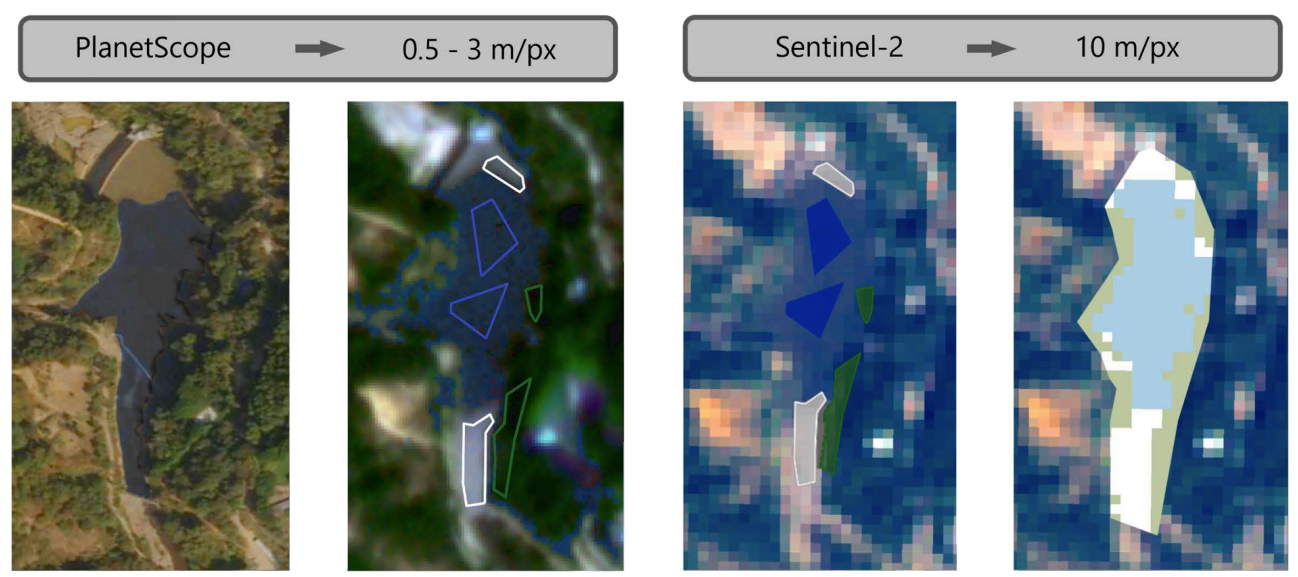
\includegraphics[width=\textwidth]{figures/perez2026.png}
        \caption{Litter likelihood estimation in river systems from Sentinel-2 and PlanetScope imagery \citepPIRusswurm{perez2025scalable}.}
        \label{fig:preliminary_work_c}
    \end{subfigure}
    \caption{Litter monitoring expertise of PIs Ru{\ss}wurm (UoB) and Garaba (UOL), evidenced by prior methodological work using uncrewed aerial vehicles (a), bridge-based imagery (b), and satellite sensors (c).}
    \label{fig:preliminary_work}
\end{figure}

\section{Objectives and work program}

\textbf{The overarching aim} of this project is to establish the scientific and methodological foundations for robust, uncertainty-aware, multiscale monitoring of riverine \textsl{macroplastic litter} by integrating experimental field observations and non-experimental Earth observation data into a unified Bayesian monitoring framework.

The project investigates the \textbf{central hypothesis} that reliable basin-scale monitoring of riverine macroplastic litter becomes possible only when treated as a \textsl{multiscale, multimodal inference problem} in which experimentally grounded local observations and non-experimental large-scale geospatial observations are explicitly aligned, calibrated, and fused. The project tests whether such fusion yields posterior estimates of litter occurrence and annual throughput that are more reliable than isolated modality-specific monitoring approaches.

\subsection{Anticipated total duration of the project}

36 Months (3 years) investigated through two PhD Projects.

\subsection{Objectives}

\begin{figure}[!h]
    \centering
    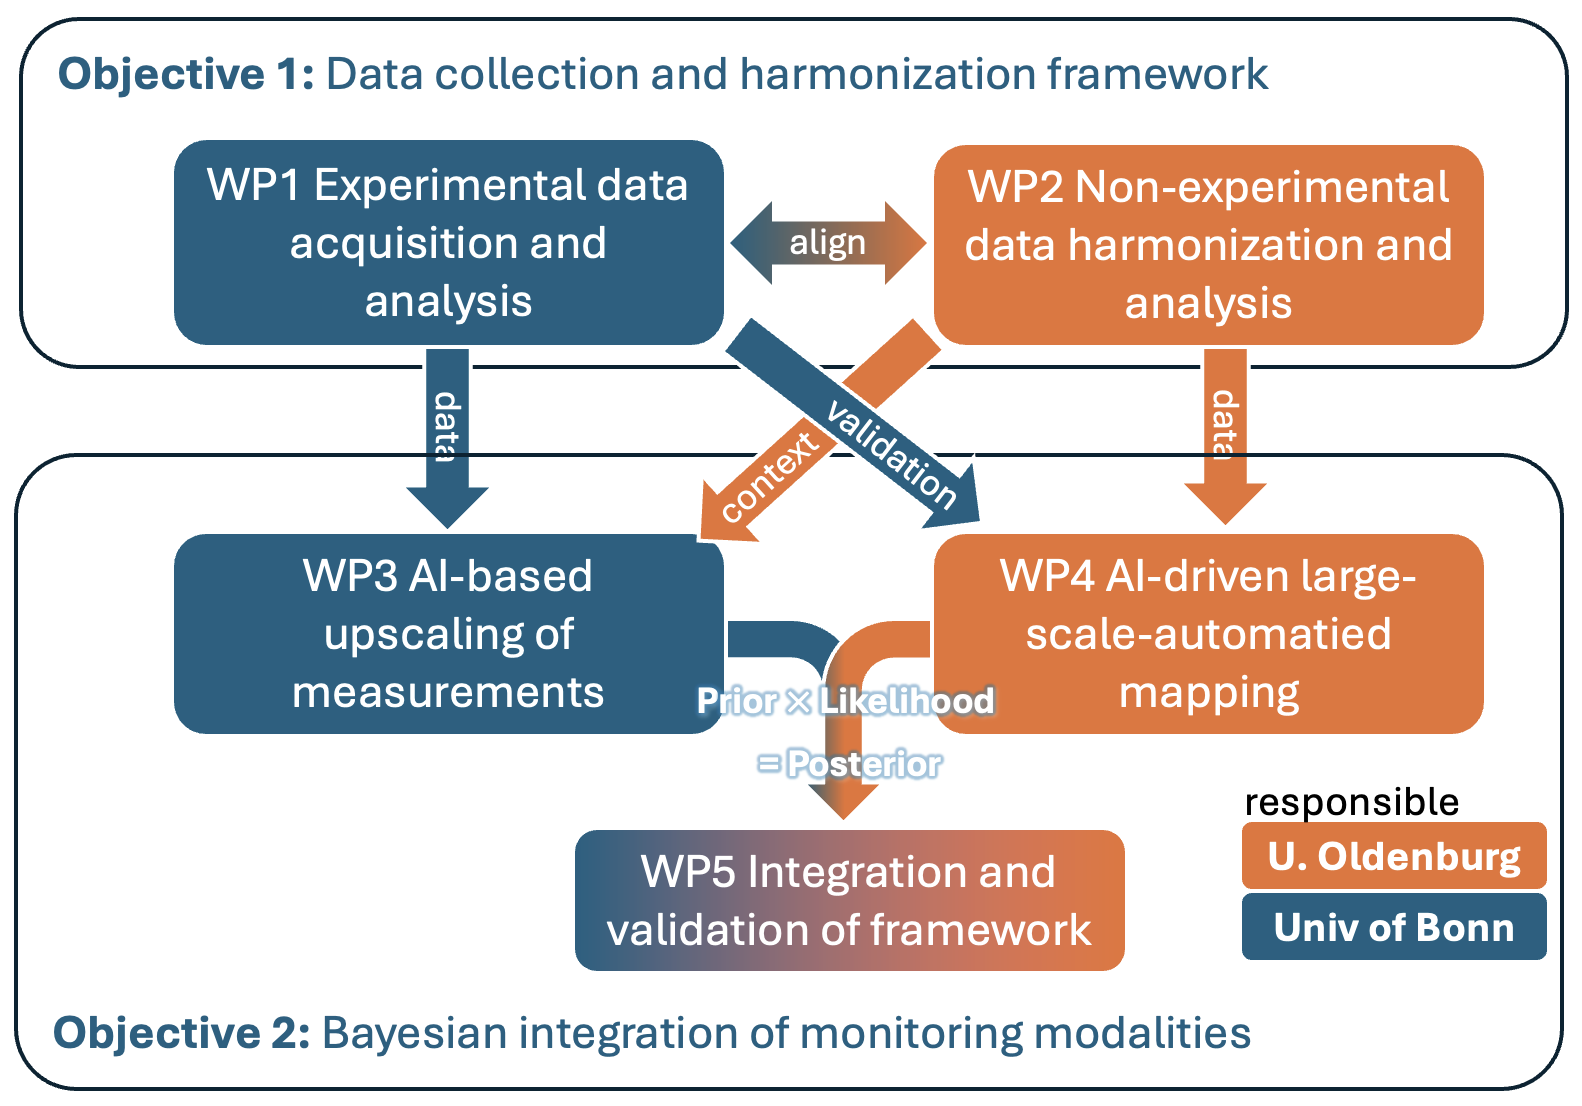
\includegraphics[width=.75\textwidth]{figures/wps.png}
    \caption{Overall structure of objectives and work packages. Objective~1 (WPs~1--2) covers experimental data acquisition and non-experimental data harmonization and analysis. Objective~2 (WPs~3--5) develops AI-based upscaling, large-scale automated mapping, and Bayesian integration into a unified monitoring framework for riverine macroplastic litter.}
    \label{fig:wps}
\end{figure}

The project addresses its overarching aim through two tightly connected objectives (Figure~\ref{fig:wps}). Objective~1 establishes the multiscale observational foundation of the project, while Objective~2 builds the uncertainty-aware AI and Bayesian framework on top of this harmonized data basis.

\begin{description}
    \item[\textbf{Objective 1: Data collection and harmonization framework (WPs~1--2)}] establishes a harmonized observational basis for riverine macroplastic monitoring by generating, assembling, and aligning complementary experimental and non-experimental data streams across scales. WP1 provides high-confidence but spatially sparse field observations of floating and stranded macroplastic litter through bridge-mounted cameras, UAV surveys, and ship-based image acquisition. WP2 complements these data with non-experimental large-scale Earth observation and contextual information, including satellite imagery, airborne and hyperspectral observations, hydrological time series, and geospatial layers along the Rhine corridor. Together, both work packages align heterogeneous data in space, time, semantics, and uncertainty characterization, thereby linking localized field evidence with basin-scale environmental context.

    \item[\textbf{Objective 2: Bayesian integration of monitoring modalities (WPs~3--5)}] develops an uncertainty-aware modelling framework that translates the harmonized data basis from Objective~1 into probabilistic monitoring products for the Rhine corridor. WP3 learns spatially explicit prior estimates of litter occurrence from sparse but high-confidence field observations and their environmental context. WP4 derives modality-specific observation likelihoods from large-scale Earth observation data. WP5 integrates both components into posterior estimates of litter presence, quantity, and hotspot probability, while validating, calibrating, and propagating uncertainty across sensors, scales, and environmental conditions. This objective tests the hypothesis that Bayesian fusion of experimentally grounded priors and observation-driven likelihoods yields more reliable and transferable basin-scale monitoring products than either branch alone.
\end{description}

This proposal does not aim to implement an operational end-user monitoring system within the project duration. Instead, it develops the scientific and methodological foundations of such a framework by establishing harmonized observations, probabilistic prior and likelihood models, and a Bayesian integration strategy with explicit uncertainty quantification. Success is therefore measured primarily in terms of methodological validity, calibration, transferability, and uncertainty-aware inference rather than full operational deployment.

\subsection{Work program including proposed research methods}
%For each applicant

%%%%%%%%%%%%%%%%%%%%%%%%%%%%%%%%%%%%%%%%%%%%%%%%%%%%%%%%%%%%%%%%%%%%%%%% 
%%%%% BEGIN OF WORK PACKAGES %%%%%%%%%%%%%%%%%%%%%%%%%%%%%%%%%%%%%%%%%%%
%%%%%%%%%%%%%%%%%%%%%%%%%%%%%%%%%%%%%%%%%%%%%%%%%%%%%%%%%%%%%%%%%%%%%%%% 
%\titlespacing*{\paragraph}{0pt}{-0.2\baselineskip}{0.2\baselineskip}
%\newcommand\WP{WP\arabic{paragraph}}

%numbered sub-workpackages are supported - just use \subparagraph{}
\RedeclareSectionCommand[indent=0pt, beforeskip=-3.5ex plus-1ex minus -.2ex,%
afterskip=2.5ex plus 0.2ex minus 0.2ex]{subparagraph}
%%%%%%%%%%%%%%%%%%%%%%%%%%%%%%%%%%%%%%%%%%%%%%%%%%%%%%%%%%%%%%%%%%%%%%%%%%%%%


%=========================================================
% Work packages (DFG Sachbeihilfe) aligned with H1--H3
%=========================================================

\subsubsection{Work package 1: Experimental field observations of floating and stranded riverine plastic litter (University of Bonn)}

\begin{figure}
    \centering
    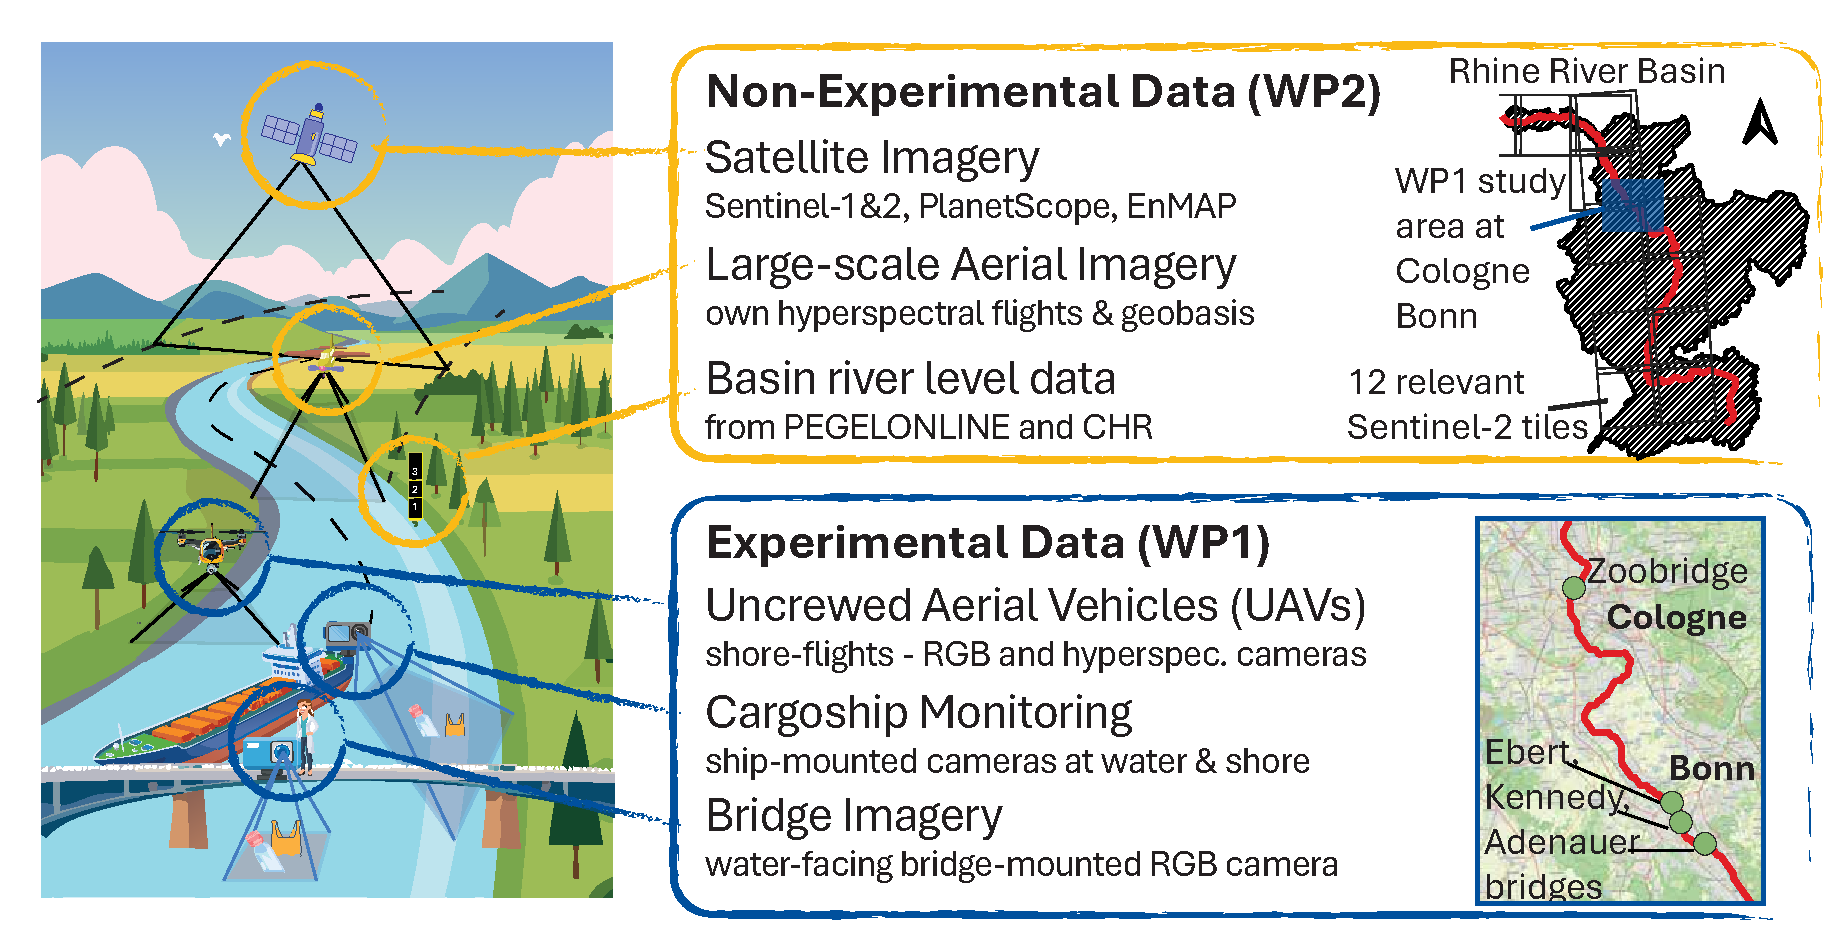
\includegraphics[width=\linewidth]{figures/Objective1.pdf}
    \caption{Overview of the planned experimental (WP1) and non-experimental (WP2) data collection and harmonization efforts for Objective~1 across the Rhine basin, with experimental studies concentrated in the Cologne/Bonn area.}
    \label{fig:dataacquisition}
\end{figure}

WP1 establishes the experimental observation backbone of the project by collecting targeted, high-quality field data on riverine macroplastic litter across complementary spatial scales. The work package is primarily focused on the Cologne/Bonn area, where logistical proximity enables repeated and temporally dense monitoring under controlled observational settings. In contrast to the large-scale geospatial datasets assembled in WP2, which exist independently of the project, WP1 focuses exclusively on observations that are generated specifically for this proposal through dedicated field campaigns, temporary instrumentation, and manual or AI-supported quantification. These measurements provide high-confidence evidence on litter occurrence, concentration, and composition at selected sites and times, and form the empirical basis for subsequent work on AI-based upscaling, automated mapping, and uncertainty-aware integration.

WP1 combines three complementary observation modalities.
\begin{description}
    \item[Bridge cameras and counting] Bridge-based camera observations and visual counting campaigns are conducted at selected monitoring sites along the Rhine, primarily around Bonn and Cologne. The planned sites include the Zoobrücke in Cologne as well as the Friedrich-Ebert-Brücke, Konrad-Adenauer-Brücke, and Kennedybrücke in Bonn. Cameras mounted on bridges, including suspended systems such as 360-degree cameras observing the water surface below, are used to record the local river section and quantify floating litter passing underneath the bridge. These observations provide point measurements of litter transport at precisely known locations and times and can be complemented by manual counting protocols and site-specific monitoring notes to create highly reliable local estimates. The Zoobrücke in Cologne is of particular importance because it enables alignment with the litter trap system reported by \cite{gnann2026river}, which is expected to remain operational during the project period. We are in contact with the KRAKE association, which coordinates the litter trap, to facilitate this linkage between camera-based observations and independent local reference measurements. The bridge camera setup and counting protocol will build on the monitoring configuration previously tested in Bangkok by \citepPIRusswurm{hagenbeek5841770exploring}, thereby grounding the data collection in an established observational workflow, including AI-based litter object detection as illustrated in \cref{fig:plastichyacinths}.

    \item[Uncrewed aerial vehicle (UAV) flights] UAV-based surveys are conducted on a semi-regular basis along selected shorelines and litter hotspots in the Cologne--Bonn area. These surveys target stranded macroplastic litter in two complementary situations: (a) highly localized and short-lived litter hotspots that emerge under suitable water-level conditions, and (b) larger shoreline sections, floodplain grasslands, and vegetated riparian areas where litter is deposited after high water levels recede. UAV imagery is particularly well suited to capture these accumulation zones at very high spatial resolution and thereby complements the bridge observations in an important way: while bridge-mounted cameras observe litter that remains in transport within the open water, UAV surveys capture litter that has already been trapped and deposited along the shore. Together, these two modalities represent distinct but connected compartments of the riverine litter system. Because these litter accumulations are highly dynamic in space and time, UAV surveys will be strongly guided by hydrological conditions, in particular water-level changes in the Rhine derived from WP2. This time-sensitive acquisition strategy will allow us to document both transient hotspot formation and post-event deposition patterns under suitable river stages. As a default platform, we will use a consumer-grade UAV equipped with an RGB camera, provided through a collaboration with Prof.\ Blanke (University of Bonn), which can be operated with minimal regulatory overhead and enables flexible short-notice deployments. For selected campaigns, we have arranged a collaboration with Prof.\ Klingbeil (University of Bonn), who can support the surveys with a larger UAV platform equipped with a hyperspectral camera. These campaigns will be designed, where possible, in temporal alignment with satellite overpasses, in particular EnMAP acquisitions in settings similar to \citep{maathuis5779542exploring}, as well as PlanetScope and Sentinel-2 observations similar to \cite{perez2025scalable}, in order to strengthen cross-scale analysis and satellite-aligned validation. \todo{Clarify which hyperspectral camera and which UAV platform will be available.}
    
    \item[Cargo ship-mounted cameras] Cameras mounted on cargo ships are used to acquire experimental observations along extended stretches of the Rhine. In contrast to the fixed bridge observations and localized UAV campaigns, ship-based image acquisition provides spatially distributed measurements along large parts of the river corridor by recording the water surface and, depending on the mounting configuration, adjacent shorelines during transit. These observations are analysed using AI-based image interpretation methods closely related to those developed for the bridge data and provide a means to extend experimental observations beyond a few local sites toward much broader coverage of the Rhine. To enable this component, we have arranged collaborations with Rhenus Logistics and Contargo GmbH to mount up to three cameras on one of their cargo ships (\cref{fig:cargoship}). The vessel regularly operates along the Rhine corridor from the Swiss border to Rotterdam and therefore offers a unique opportunity to acquire in-situ visual observations across a large fraction of the study area. We will explore two complementary camera configurations. First, water-facing cameras will record the river surface to capture floating litter and sediments, but also surface properties such as turbidity and water colour. These observations are relevant not only for direct litter monitoring, but also for the verification and validation of the spectral Earth observation measurements assembled in WP2. In this way, while bridge-mounted cameras and UAV surveys remain localized to the Cologne--Bonn area, the cargo ship observations provide distributed near-surface reference data along much larger parts of the Rhine. Second, we will investigate shore-facing camera configurations that may capture litter hotspots and trapped shoreline litter, where debris often remains visible for longer periods than in open water. Because such acquisitions raise privacy concerns, this setup will only be pursued under strict data protection procedures. In particular, image data will be anonymized as early as possible after acquisition to mitigate privacy risks while preserving their scientific value for litter monitoring.
\end{description}

\begin{figure}
    \centering
    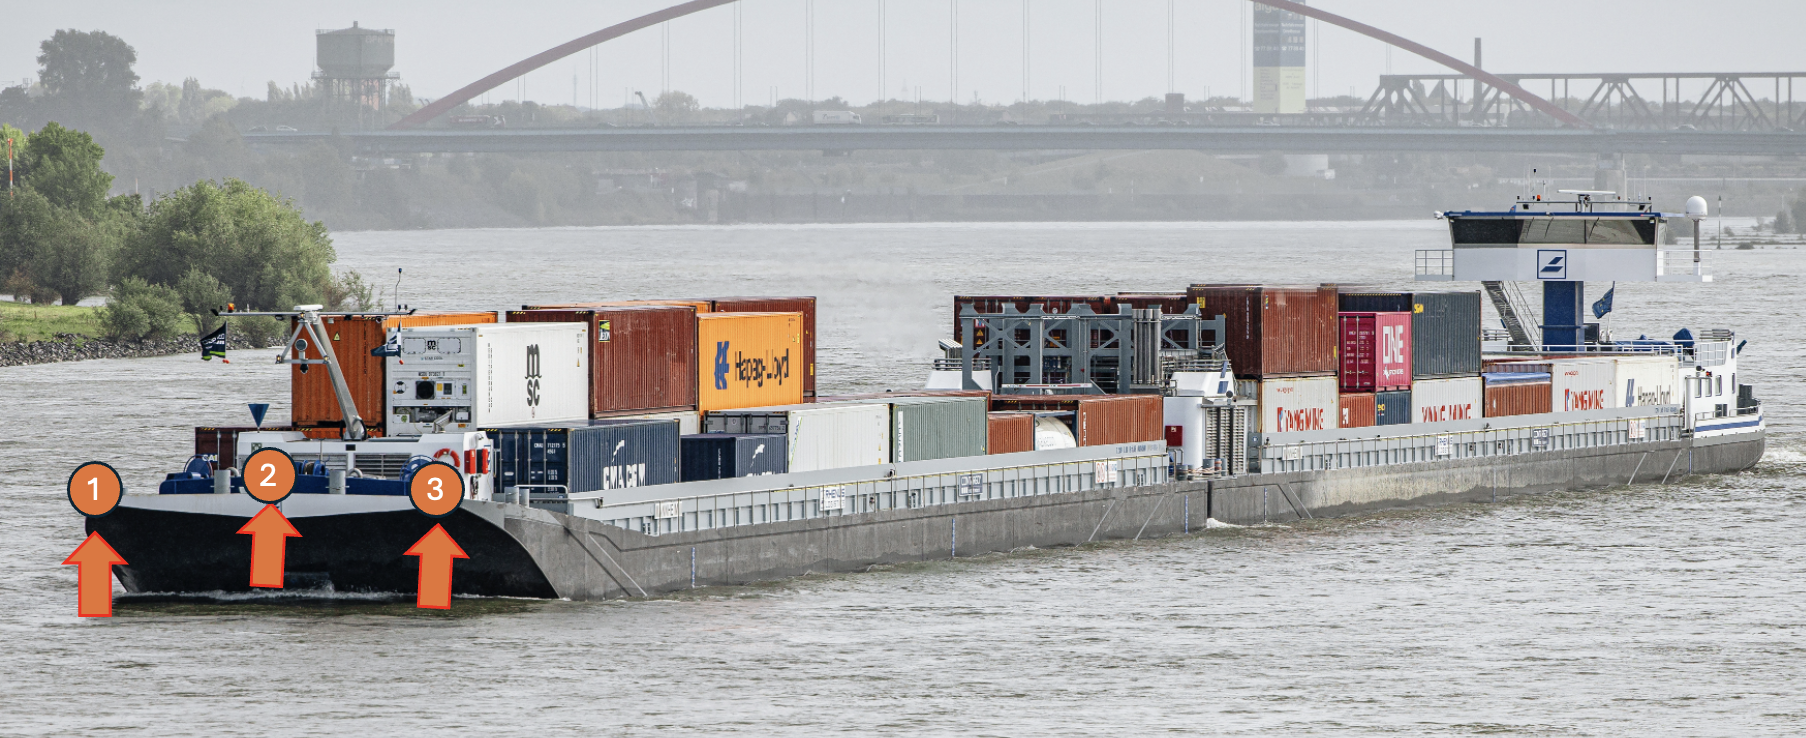
\includegraphics[width=0.67\linewidth]{figures/cargoship.png}
    \hfill
    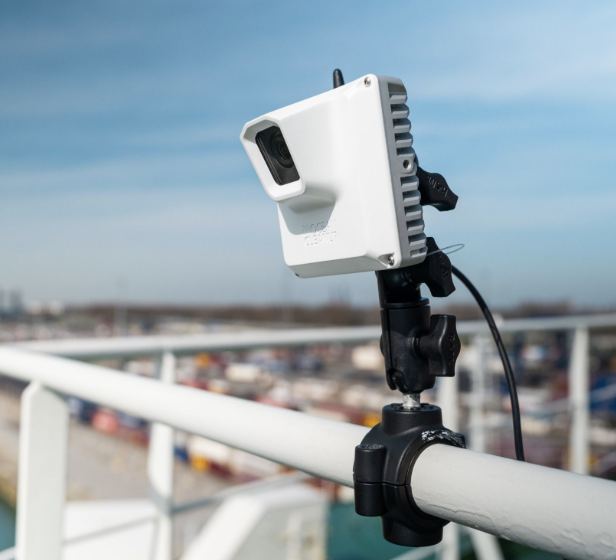
\includegraphics[width=0.302\linewidth]{figures/adis.png}
    \caption{Left: Planned mounting arrangement of up to three cameras on the cargo ship selected for this study, optimally with two shore-facing cameras and one water-facing camera. The vessel is operated by Rhenus Logistics and Contargo GmbH. Right: The Automated Debris Imaging System (ADIS) developed by The Ocean Cleanup, which uses AI-powered cameras to collect surface imagery.}
    \label{fig:cargoship}
\end{figure}

\textbf{Deliverables} The main deliverables of WP1 are, first, the harmonization of the three observational streams into a common experimental dataset with standardized metadata, annotation protocols, and modality-specific uncertainty descriptors, and second, a comparative suitability and uncertainty assessment across the three data modalities. The harmonized dataset will systematically record site characteristics, sensor geometry, acquisition conditions, and the distinction between floating and stranded litter compartments. Over the three-year project period, WP1 will thereby generate a geolocated experimental dataset centered on the Cologne--Bonn area through bridge and UAV observations, complemented by cargo ship image acquisitions along the Rhine corridor from the Swiss border to Rotterdam.

\textbf{Links to follow-up WPs} The comparative suitability assessment will quantify the strengths, limitations, and error characteristics of bridge-mounted cameras, UAV surveys, and cargo ship-mounted cameras, for example in the form of confusion matrices and related reliability measures. These modality-specific uncertainty estimates will be essential for calibrating the relative trustworthiness of each data source in the joint Bayesian framework developed in WP3--WP5. In this way, WP1 provides the experimentally grounded evidence base on which the later AI-based upscaling, automated mapping, and Bayesian data fusion components of the project can be calibrated and validated.

\textbf{Evaluation and success criteria.} Success in WP1 will be measured by whether the experimental observations provide a temporally repeated, spatially localized, and quality-controlled reference basis for later modelling work. This includes consistent georeferencing and time stamping across bridge, UAV, and ship-based acquisitions, sufficient coverage of contrasting hydrological and observational conditions, and the derivation of reliable reference observations on litter occurrence, concentration, and composition. WP1 is successful if it yields a robust validation and calibration basis for the methodological developments in WPs 3--5.


\subsubsection{Work Package 2: Large-scale Earth observation and geospatial database of the Rhine corridor (University of Oldenburg)}

WP2 establishes the non-experimental data backbone of the project by assembling, harmonizing, and curating large-scale Earth observation and contextual datasets across the Rhine basin, primarily on the German side and downstream toward the Netherlands. In contrast to WP1, which generates targeted experimental observations through dedicated field campaigns and temporary instrumentation, WP2 focuses on non-experimental data streams that already exist independently of the project and can therefore provide broad spatial coverage, temporal continuity, and retrospective depth. These datasets describe the Rhine river corridor over space and time and provide the contextual and observational basis for subsequent large-scale AI-based mapping and integrated uncertainty-aware monitoring.

WP2 combines four complementary data modalities.
\begin{description}
    \item[Sentinel-2 and PlanetScope] A primary component of WP2 is the compilation and preprocessing of multispectral satellite imagery along the Rhine corridor, including a buffer of approximately 2\,km on both sides of the river. The focus is on harmonizing multi-year archives of Sentinel-2 observations over the main study region, complemented where available by higher-resolution PlanetScope imagery. Relevant Sentinel-2 MGRS tiles for this study area include 31UET, 31UFT, 31UGS, 31UGT, 32TLT, 32TMT, 32ULA, 32ULB, 32ULC, 32ULU, 32UMA, 32UMU, and 32UMV. Together, these data provide broad temporal coverage and improved spatial detail for characterizing river sections, shoreline appearance, adjacent land cover, and potential litter-related surface patterns. \todo{Shungu: add details on temporal depth, preprocessing, atmospheric correction, cloud handling, and the complementary roles of Sentinel-2 and PlanetScope.}

    \item[EnMAP acquisitions] WP2 further integrates spaceborne hyperspectral observations from EnMAP to complement the multispectral archive with richer spectral information. These data are particularly relevant for assessing the spectral detectability of plastics and related materials under varying environmental conditions and for linking satellite observations more directly to the material-oriented interpretation developed in the project. EnMAP acquisitions will be used where available across the Rhine corridor and, where possible, aligned with targeted UAV and airborne campaigns from WP1 and WP2 to enable cross-scale comparison. \todo{Shungu: specify acquisition strategy, expected number of scenes, spectral preprocessing, and the role of EnMAP for plastic detectability and transfer across sensors.}

    \item[Water level data] WP2 includes hydrological context data, in particular river water levels and related descriptors relevant to plastic transport, accumulation, shoreline exposure, and post-event deposition. These variables are essential for interpreting when and where litter is likely to be mobilized, transported, stranded, or visible to remote sensing systems. Water-level time series will therefore be linked to both the satellite archive and the experimental observations from WP1 in order to provide temporal environmental context for hotspot formation, deposition events, and changing detectability conditions. \todo{Specify the hydrological data sources, e.g.\ PEGELONLINE and related Rhine gauge products, and describe which derived variables will be included.}

    \item[Aerial flights] In addition to satellite-based observations, WP2 includes targeted airborne remote sensing campaigns using hyperspectral sensors mounted on aircraft. These flights are conducted approximately once per year over selected river sections and provide high-resolution imaging spectroscopy data that bridge the gap between local field observations and satellite-scale measurements. They complement EnMAP observations by offering substantially finer spatial detail than current spaceborne hyperspectral sensors and therefore support the analysis of spectral detectability, sensor transfer, and scale effects. \todo{Shungu: add details on flight partners, sensor specifications, planned river sections, and alignment with EnMAP and WP1 acquisition windows.}
\end{description}

\textbf{Deliverables} The main deliverables of WP2 are, first, the harmonization of these non-experimental data streams into a common geospatial database with standardized metadata, spatial references, temporal alignment, and modality-specific quality descriptors, and second, a curated spatial-temporal data cube of the Rhine corridor integrating multispectral and hyperspectral satellite observations, airborne hyperspectral campaigns, hydrological time series, and relevant contextual GIS layers. This database will systematically describe the river environment, adjacent infrastructure and land use, and the temporal environmental conditions relevant to litter occurrence, transport, deposition, and visibility.

\textbf{Links to follow-up WPs} WP2 provides the large-scale observational and environmental context required for the subsequent methodological work packages. In WP3, these data serve as contextual information for spatially informed upscaling of the experimentally grounded observations from WP1. In WP4, they provide the primary input for AI-based automated mapping from Earth observation data at larger scales. Within the Bayesian integration framework of WP3--WP5, WP2 therefore contributes the non-experimental context and likelihood-related observation basis that complements the experimentally grounded validation and calibration evidence generated in WP1.

\textbf{Evaluation and success criteria.} Success in WP2 will be measured by whether the non-experimental Earth observation and geospatial database is harmonized, reproducible, and sufficiently complete to support basin-scale analysis. This includes coherent preprocessing across satellite, airborne, hydrological, and GIS data sources, alignment in space and time with WP1 observations wherever possible, and transparent documentation of coverage, uncertainty, and data gaps. WP2 is successful if it provides a reusable and analysis-ready geospatial database that can support both prior learning in WP3 and image-based likelihood modelling in WP4.


\subsubsection{Work Package 3: Geospatial embedding and prior modelling for AI-based upscaling}

\begin{figure}[!h]
    \centering
    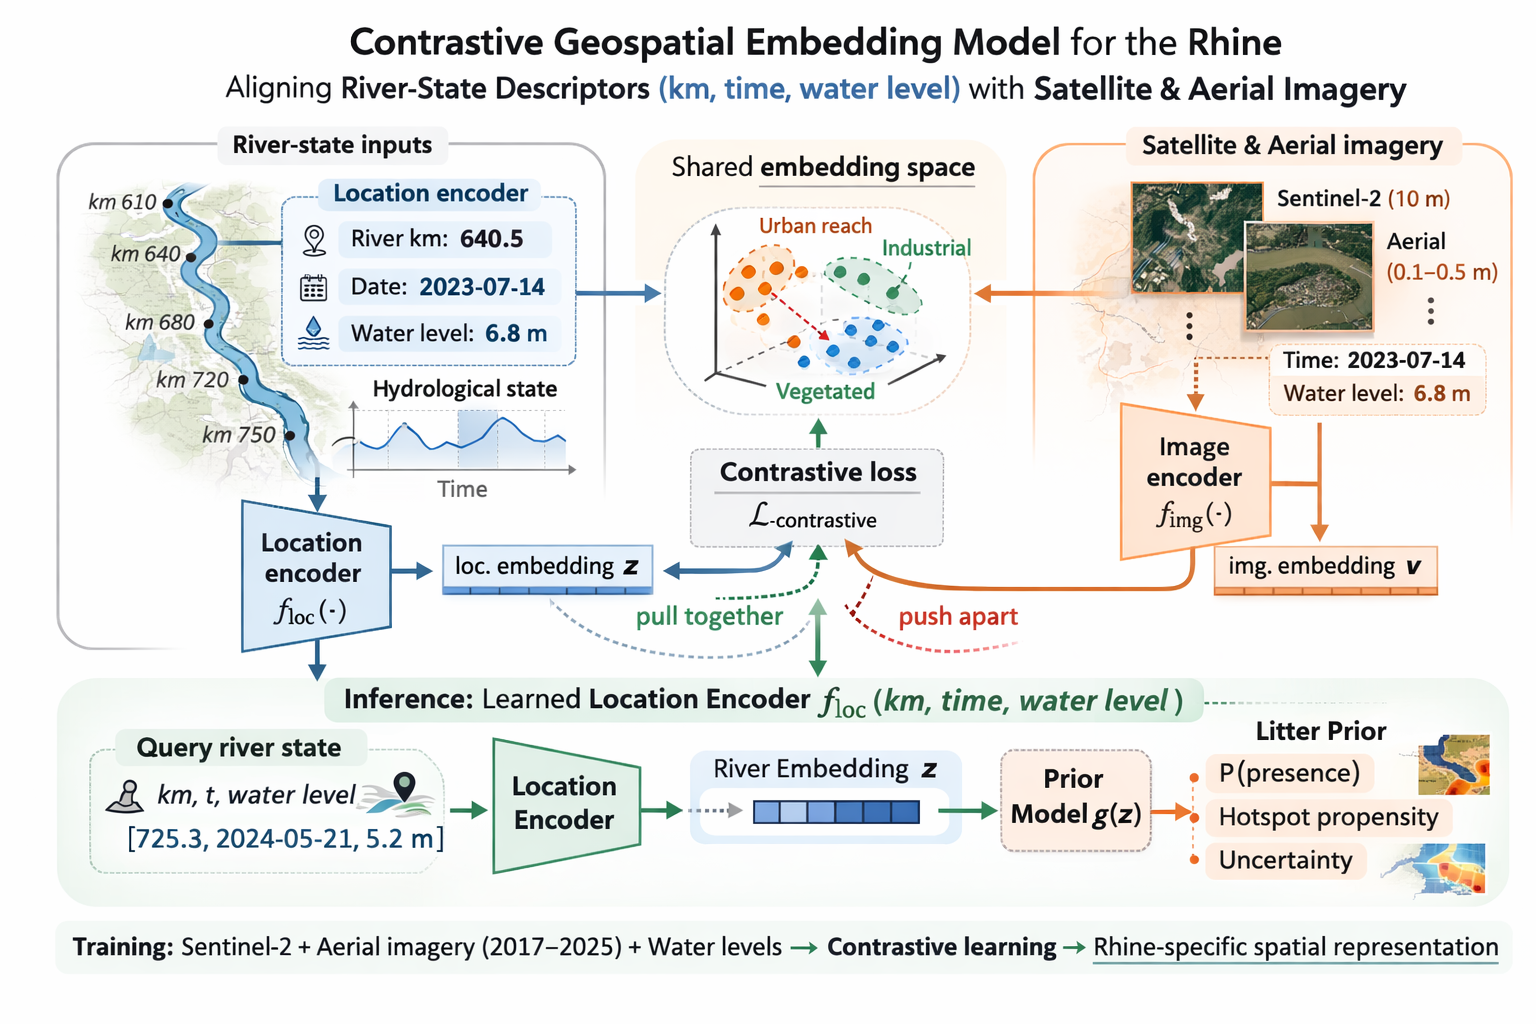
\includegraphics[width=\linewidth]{figures/RiverCLIP.png}
    \caption{Schematic overview of the contrastive geospatial embedding model in WP3. A Rhine-specific location encoder, parameterized by river kilometer, time, and water level, is trained jointly with an image encoder on corresponding satellite and aerial imagery to learn a shared embedding space. The learned location encoder then serves as a continuous representation of the Rhine that supports prior modelling of litter presence and hotspot propensity. Figure adapted to river setting from originally global SatCLIP model \citepPIRusswurm{klemmer2025satclip}.}
    \label{fig:RiverCLIP}
\end{figure}

WP3 develops a Rhine-specific geospatial embedding model that learns a continuous representation of the river corridor as a function of river-aligned position, time, and hydrological state. Inspired by recent work on contrastive geospatial representation learning and AI-centric Earth representations \citep{klemmer2025satclip,klemmer2025earth}, the model is trained to align a location encoder, parameterized by kilometer marker, date, and water level, with corresponding Sentinel-2 and high-resolution aerial imagery in a shared embedding space. The resulting location encoder serves as an implicit model of the Rhine that captures recurring spatial, seasonal, and hydrological patterns such as urbanized reaches, industrial corridors, vegetated shorelines, or flood-prone accumulation zones. By linking this learned environmental representation to the experimentally observed litter occurrences from WP1, WP3 derives a spatially continuous prior model of litter presence and hotspot propensity that can be queried for arbitrary river sections, times, and water levels, even in the absence of direct observations.

\textbf{Proposed research methods.} WP3 uses the harmonized observational and contextual database established in Objective~1, combining sparse but high-confidence litter observations from WP1 with the large-scale Earth observation and hydrological context assembled in WP2. The core training data consist of multi-temporal Sentinel-2 imagery from 2017 onward, complemented by high-resolution aerial imagery from Geobasis NRW, together with river-aligned kilometer markers, acquisition dates, and water-level information derived from the hydrological time series. Based on these inputs, WP3 develops a contrastive geospatial representation learning framework inspired by SatCLIP-like models \citep{klemmer2025satclip}, in which a location encoder parameterized by river kilometer, time, and hydrological state is trained jointly with an image encoder to map both modalities into a shared latent space. In contrast to global coordinate encoders that operate directly on longitude and latitude, the proposed model adopts a river-aligned parameterization tailored to the one-dimensional topology and dynamics of the Rhine, while conceptually building on recent work on continuous geographic location encoding and implicit embedding models \citep{russwurm2024geographic,klemmer2025earth}. In this way, the model learns a continuous semantic representation of the Rhine that organizes river sections according to recurring environmental and morphological patterns relevant for litter occurrence, transport, and deposition. In a second step, this learned embedding space is linked to the experimentally observed floating and stranded litter occurrences from WP1 in order to infer spatial litter priors and hotspot propensity from environmental similarity. This allows the sparse field observations to be generalized beyond the directly observed sites and times toward unmonitored river reaches and hydrological conditions. Methodologically, particular emphasis is placed on uncertainty-aware prior estimation, including the quantification of representativeness, transferability, and confidence when extrapolating from observed to unobserved river states.

\textbf{Deliverables} The main deliverables of WP3 are, first, a Rhine-specific geospatial embedding model that provides a continuous representation of the river corridor as a function of location, time, and water level, and second, a spatially continuous prior model of litter presence and hotspot propensity derived from the linkage between this embedding space and the experimental observations from WP1. Additional deliverables include a river-wide embedding data product for the Rhine corridor, representativeness and uncertainty layers indicating where prior estimates are well supported by observed environmental analogues, and an evaluation of how well the learned representation supports transfer across river sections, seasons, and hydrological conditions. Together, these outputs provide the prior component required for the subsequent Bayesian integration in WP5.

\textbf{Links to other WPs} WP3 builds directly on both observational streams established in Objective~1. WP1 provides the experimentally grounded litter observations required to relate the learned embedding space to actual litter occurrence, while WP2 provides the large-scale Earth observation, hydrological, and geospatial context from which the Rhine representation is learned. In contrast to WP4, which derives observation-based likelihood information from large-scale sensing data, WP3 provides a contextual prior of where litter is expected to occur based on environmental, seasonal, and hydrological similarity. The resulting prior model forms one of the two core probabilistic components of the overall monitoring framework and is integrated with the likelihood estimates from WP4 in WP5 to produce posterior estimates of litter presence, quantity, and hotspot probability along the Rhine.

\textbf{Evaluation and success criteria.} Success in WP3 will be measured by whether the learned contextual prior captures meaningful spatial and environmental structure beyond simple interpolation or heuristic hotspot mapping. Evaluation will focus on the ability of the prior model to generalize from sparse experimentally grounded observations to unseen river sections and conditions, while remaining interpretable with respect to hydrological, seasonal, and geospatial context. WP3 is successful if it produces spatially explicit prior estimates that improve hotspot ranking, transferability, and uncertainty-aware initialization for posterior inference in WP5.


\subsubsection{Work Package 4: Multi- and hyperspectral large-scale litter analysis for the Rhine basin (University of Oldenburg)}

WP4 develops the large-scale remote-sensing component of the project by estimating the likelihood of riverine macroplastic litter presence directly from Earth observation imagery. In contrast to WP3, which learns a contextual prior of where litter is expected to occur from geospatial and hydrological similarity, WP4 focuses on observation-driven evidence extracted from multi- and hyperspectral data. Building on the harmonized satellite, airborne, and contextual database assembled in WP2, WP4 develops AI-based mapping methods that infer litter likelihood from individual image acquisitions at larger spatial scales. In this way, WP4 translates Earth observation data into the likelihood component of the Bayesian monitoring framework, providing image-based evidence of litter presence that can later be integrated with the prior estimates from WP3 in WP5.

\textbf{Proposed research methods.} WP4 uses the multi- and hyperspectral Earth observation data assembled in WP2, including Sentinel-2, PlanetScope, EnMAP, and airborne hyperspectral imagery, together with the experimental reference observations from WP1 for validation and calibration. Methodologically, the work package develops image-based models that estimate the probability of litter presence from a given image acquisition, while explicitly accounting for differences in spatial resolution, spectral richness, viewing geometry, and environmental conditions. The work builds on recent AI-based remote-sensing approaches for debris and litter analysis, including large-scale pixel-wise debris detection from Sentinel-2 \citep{russwurmcell2023} and the use of segment-anything-based workflows for spectral-index search and debris visualization \citepPIRusswurm{van2025samselect}. A central objective is to move from image interpretation toward probabilistic litter-likelihood estimation, such that each image yields a calibrated likelihood of litter presence rather than only a hard detection. Methodological development will therefore include multimodal and multisensor learning strategies, sensor-aware calibration, and explicit treatment of detectability limits across environmental conditions. \todo{Shungu: specify which sensors and combinations will form the main methodological core of WP4, e.g.\ Sentinel-2 only, Sentinel-2 + EnMAP, or airborne-to-spaceborne transfer settings.} \todo{Shungu: add the role of hyperspectral analysis for resolving spectral ambiguities between plastics, foam, wood, vegetation, sediment, and other optically similar materials.} \todo{Shungu: describe whether the work will focus on pixel-wise segmentation, object detection, weak supervision, spectral unmixing, anomaly detection, or a combination thereof.} \todo{Shungu: add details on the use of annual aerial campaigns and EnMAP-aligned acquisitions for cross-scale transfer and sensor benchmarking.} \todo{Shungu: clarify how water level, turbidity, seasonality, and shoreline background will enter the modelling or evaluation as factors affecting detectability and confidence.}

\textbf{Deliverables} The main deliverable of WP4 is an AI-based mapping methodology that estimates the likelihood of litter presence from a single multi- or hyperspectral image and thereby provides the likelihood component required for the Bayesian integration in WP5. Additional deliverables include calibrated image-based litter-likelihood products for selected Rhine sections and acquisition dates, as well as a systematic evaluation of model performance and uncertainty across sensors, seasons, and hydrological conditions. \todo{Shungu: specify which concrete model outputs will be delivered, e.g.\ pixel-level likelihood maps, section-level likelihood scores, hotspot rankings, or aggregated river-section summaries.} \todo{Shungu: add expected deliverables on hyperspectral detectability analysis, cross-sensor transferability, and interpretability of spectral signatures.} \todo{Shungu: clarify whether the work package will deliver benchmark datasets, annotated validation subsets, or sensor comparison studies as standalone outputs.}

\textbf{Links to other WPs} WP4 builds directly on the non-experimental Earth observation and geospatial database assembled in WP2 and uses the experimentally grounded observations from WP1 for validation and calibration of image-based litter estimates. In conceptual terms, WP4 complements WP3: whereas WP3 provides a contextual prior of where litter is expected to occur based on the learned semantic and hydrological similarity of river states, WP4 provides observation-based likelihood information derived from actual image acquisitions. The outputs of WP4 therefore form the second core probabilistic component of the overall monitoring framework and are combined with the prior estimates from WP3 in WP5 to produce posterior estimates of litter presence, quantity, and hotspot probability along the Rhine.

\textbf{Evaluation and success criteria.} Success in WP4 will be measured by whether the image-based models provide calibrated and transferable estimates of litter likelihood across sensors, seasons, and environmental conditions. Evaluation will consider predictive performance as well as robustness to domain shifts caused by water level, turbidity, illumination, shoreline background, and sensor characteristics. WP4 is successful if it yields observation-based likelihood estimates with quantified confidence that complement the contextual prior from WP3 and can be consistently integrated in WP5.

\subsubsection{Work Package 5: Bayesian integration and uncertainty-aware monitoring framework (joint University of Bonn and University of Oldenburg)}

WP5 is the final integrative work package of the project and the key step in testing the central hypothesis. Building on the multiscale observational basis established in WPs~1--2, the contextual prior model learned in WP3, and the modality-specific observation likelihoods derived in WP4, WP5 develops the first cohesive multimodal Bayesian monitoring framework of the project. This integration is the central methodological innovation of the proposal. Existing approaches largely remain limited to separate sensor- or modality-specific likelihood estimates, for example from individual satellite, hyperspectral, aerial, or image-based detection pipelines, without combining them consistently with contextual prior information and uncertainty into a unified posterior estimate. WP5 addresses this gap for riverine macroplastic litter monitoring along the Rhine.

\textbf{Proposed research methods.} At its core, WP5 formulates multimodal litter monitoring as a Bayesian posterior inference problem in which a contextual prior is updated with modality-specific observation likelihoods:
\[
\underbrace{\overset{\mathbf{WP5}}{p(z \mid \mathcal{Y})}}_{\text{posterior monitoring estimate}}
\;\propto\;
\underbrace{\overset{\mathbf{WP3}}{p(z \mid \mathbf{c})}}_{\text{contextual prior}}
\cdot
\underbrace{\overset{\mathbf{WP4}}{\prod_{m \in \mathcal{M}} p\!\left(\mathbf{y}^{(m)} \mid z\right)}}_{\text{modality-specific likelihoods}}.
\]
Here, \(z\) denotes the latent litter state of interest, \(\mathbf{c}\) summarizes contextual covariates such as river kilometer, water level, and day of year, and \(\mathcal{Y}\) denotes the set of available observations from sparse sensing modalities such as Sentinel-2, PlanetScope, EnMAP, and aerial flights. The methodological development of WP5 is structured into five blocks:

\begin{description}
    \item[\textbf{(1) Inference target and spatial support.}] WP5 investigates two linked posterior targets. The primary target is a spatially continuous posterior estimate of litter occurrence along the Rhine, represented as a function of river position and contextual conditions rather than as a fixed raster product. This supports hotspot identification and localized litter quantification and can be validated against experimentally grounded observations from WP1 and aligned with external monitoring activities such as RhineKrake. The second target is an aggregated uncertainty-aware estimate of annual litter throughput for the Rhine, intended to constrain the large discrepancy between published Rhine-wide estimates ranging from 65~tpy \citep{van2022hydrology} to 4000~tpy \citep{gnann2026river}. Inference is carried out on a continuous river support parameterized by river kilometer, allowing posterior estimates to be queried at arbitrary locations and aggregated over river sections, monitoring sites, or annual basin-wide summaries.

    \item[\textbf{(2) Bayesian fusion of sparse multimodal observations.}] The core methodological contribution of WP5 is the fusion of sparse and asynchronous sensing modalities into a shared posterior estimate. For a given river location and time, the contextual prior from WP3 is updated with the subset of modality-specific likelihoods available from WP4, without requiring synchronous coverage across all sensors. Because all sensing streams provide complementary evidence about the same latent litter state, this setting naturally motivates product-of-experts-style fusion, in which each available modality acts as a probabilistic expert whose contribution sharpens the posterior when informative evidence is present \citep{hinton1999temporal}. WP5 will investigate calibrated product-of-experts formulations, as well as hierarchical Bayesian and Gaussian-process-based variants that support smooth uncertainty-aware interpolation under incomplete observation coverage.

    \item[\textbf{(3) Calibration and uncertainty propagation.}] WP5 integrates uncertainty information at two complementary levels. First, calibration studies from WPs~1 and 2 provide modality-level reliability information, for example through confusion matrices, error statistics, and condition-specific performance analyses for Sentinel-2, PlanetScope, EnMAP, bridge imagery, and related sensing streams. These empirical reliability estimates are used to calibrate and harmonize modality-specific likelihoods before fusion. Second, the underlying models are extended with observation-level uncertainty estimates for individual acquisitions, for example using deep ensembles, Monte Carlo dropout, or evidential approaches based on Dirichlet output distributions where appropriate. Together, these two levels allow prior uncertainty, sensor-specific reliability, and per-observation predictive uncertainty to be propagated into the posterior estimate.

    \item[\textbf{(4) Validation, ablation, and added value of fusion.}] WP5 will determine whether multimodal Bayesian fusion provides measurable benefits over simpler monitoring strategies. Validation compares prior-only, single-modality, and fused posterior estimates against experimentally grounded observations from WP1 and, where possible, external monitoring activities such as RhineKrake. Evaluation considers both predictive performance and probabilistic calibration, with particular attention to whether fusion reduces false positives, improves hotspot identification, and yields more reliable estimates under sparse or heterogeneous sensing conditions. Ablation experiments quantify the contribution of the contextual prior, modality-specific likelihoods, calibration procedures, and uncertainty estimates to final posterior performance.

    \item[\textbf{(5) Monitoring products and temporal aggregation.}] The final block translates the posterior inference framework into practical monitoring products at multiple spatial and temporal scales. At the local scale, WP5 generates spatially continuous posterior estimates of litter occurrence and hotspot probability for individual acquisitions, which can be summarized into river-section indicators and persistent hotspot maps through aggregation across space and time. At the basin scale, repeated posterior estimates are integrated into uncertainty-aware annual throughput estimates for macroplastic litter in the Rhine. A central aim is to retain uncertainty throughout this aggregation process, such that both local hotspot maps and basin-scale annual quantities are accompanied by interpretable confidence bounds.
\end{description}

\textbf{Deliverables.} WP5 delivers the unified Bayesian monitoring framework of the project, including calibrated multimodal posterior estimates that combine contextual priors and modality-specific likelihoods under incomplete observation coverage. The main outputs are spatially continuous posterior estimates of litter occurrence and hotspot probability along the Rhine, uncertainty-aware river-section summaries, and an aggregated annual estimate of Rhine-wide macroplastic litter throughput with associated confidence bounds. In addition, WP5 provides a quantitative validation and ablation analysis that assesses the added value of multimodal Bayesian fusion over prior-only and single-modality baselines.

\textbf{Links to other WPs.} WP5 is the integrative work package of the project and directly builds on all preceding components. WPs~1 and 2 provide the experimental reference observations, calibration studies, and multimodal Earth observation database that form the empirical basis for fusion and validation. WP3 contributes the Rhine-specific contextual prior model, while WP4 provides the modality-specific observation likelihoods derived from satellite, airborne, and image-based sensing streams. In turn, WP5 synthesizes these inputs into the unified posterior monitoring framework of the proposal and translates them into the final monitoring products, including spatially continuous litter-occurrence estimates, hotspot maps, and annual throughput estimates for the Rhine.

\textbf{Evaluation and success criteria.} Success in WP5 will be measured by whether Bayesian integration of contextual priors and modality-specific likelihoods yields more reliable and informative posterior estimates than either component alone. Evaluation will compare posterior predictions against experimentally grounded observations from WP1 and against reduced baselines such as prior-only, single-modality, or non-probabilistic alternatives. WP5 is successful if the resulting posterior estimates show improved calibration, uncertainty characterization, and robustness for hotspot identification, localized quantification, and constrained basin-scale inference.

\subsubsection{Scientific risks and mitigation}

The main risks of the project are scientific and arise from uncertainty in detectability, transferability, and cross-scale integration. The proposal therefore develops the scientific and methodological foundations of an uncertainty-aware monitoring framework rather than aiming at a fully operational end-user system within the project duration.

A first risk is that litter signals in satellite, airborne, or proximal imagery are weak or confounded by background conditions such as turbidity, illumination, or shoreline complexity. This is mitigated by treating image-derived estimates as modality-specific likelihoods with quantified confidence rather than as deterministic detections. If detectability is limited for some sensors or conditions, the project will still identify when and where remote sensing contributes reliable evidence.

A second risk is limited transferability across river sections, seasons, and hydrological states. This is mitigated by combining experimentally grounded observations from WP1 with the large-scale contextual database from WP2 and by learning an explicit contextual prior in WP3 rather than relying only on local interpolation. Even if generalization is weaker than expected, the project will still quantify which covariates and sensing conditions support robust transfer.

A third risk is uncertainty in linking local observations and image-based detections to section-level quantities or annual throughput. This is addressed by formulating throughput estimation as an uncertainty-aware posterior inference problem in WP5 and by using experimentally grounded observations and interception-based measurements as calibration anchors wherever possible. If the full basin-scale aggregation remains too uncertain, the project will still deliver validated hotspot estimates and river-section indicators with interpretable confidence bounds.

The proposal is robust against partial failure because each work package yields a standalone methodological contribution: harmonized multimodal observations (WPs 1--2), contextual prior modelling (WP3), calibrated image-based likelihoods (WP4), and probabilistic fusion with uncertainty propagation (WP5).

\subsection{Handling of research data}

\textbf{2.4.1 Data description.} The project will generate and integrate multimodal research data from experimental field observations and non-experimental Earth observation sources along the Rhine corridor. These include bridge-mounted and cargo-ship-based RGB imagery, UAV imagery, satellite data (e.g., Sentinel-2, PlanetScope), airborne and hyperspectral imagery (e.g., EnMAP and dedicated aerial campaigns), hydrological time series such as river level data, and associated geospatial context layers. In addition, field observations and annotations will be recorded in structured digital tables (e.g., ASCII tab-delimited files or spreadsheet formats) with standardized file names, column headers, and metadata. Raw imagery, processed data products, annotations, calibration studies, and derived monitoring outputs will be stored centrally and jointly curated across the project.

\textbf{2.4.2 Documentation and data quality.} Raw and derived data products will be organized, versioned, documented, and quality-controlled throughout the project. Metadata standards and data organization will follow established geospatial and Earth observation conventions wherever applicable. Documentation will include sensor type, acquisition time, location, preprocessing steps, annotation status, and quality flags. Calibration datasets, confusion matrices, and condition-specific performance analyses generated in the project will form part of the documented data basis and support downstream uncertainty analysis and validation. Metadata generation and data documentation will build on prior experience within the consortium, including peer-reviewed data description and open dataset publication practices established in earlier work by PI Garaba and collaborators. Derived code and processing workflows used to curate, harmonize, and analyze the data will be maintained in version-controlled repositories and made openly available where possible.

\textbf{2.4.3 Storage and technical archiving during the project.} The project budgets two dedicated data storage and processing servers hosted at the Hochschulrechenzentrum of the University of Bonn. These servers will provide the central infrastructure for joint data access, processing, and storage across the project. One server will serve as the primary storage and processing system, while the second server will act as a dedicated backup of the first. This setup ensures centralized project-wide data management, secure storage, controlled access, and redundancy for large multimodal datasets such as imagery, annotations, and derived model outputs.

\textbf{2.4.4 Legal obligations and conditions.} The project will comply with all relevant legal and ethical requirements, including the General Data Protection Regulation (GDPR), whenever applicable. Image acquisition that is exclusively directed at the water surface is considered uncritical from a data protection perspective. Where bridge- or cargo-ship-based imagery may also capture shore areas or persons, the project will implement a data protection workflow consistent with the preliminary guidance received from the University of Bonn's research data service. In such cases, the processing of potentially personal data for scientific purposes may be justified under BDSG \S27 and DSG NRW \S17, provided that appropriate safeguards are implemented. These safeguards include internal screening of raw imagery where necessary, anonymization at the earliest possible stage through masking or pixelation of sensitive areas, publication only in anonymized form, and timely deletion of problematic raw data. Fully anonymized data will no longer fall under the GDPR. The project will explicitly accommodate these requirements in its data collection and processing protocols.

\textbf{2.4.5 Data exchange and long-term accessibility.} Data exchange within the project will take place through the centrally hosted server infrastructure with controlled access for authorized project members. Curated datasets, derived products, and selected annotations will be prepared for long-term open-access publication in suitable repositories, subject to legal and ethical constraints. Wherever possible, curated and anonymized versions of the raw datasets underlying project publications will be released alongside the corresponding articles on public platforms such as Zenodo with persistent identifiers (DOIs), thereby providing a well-documented and harmonized dataset basis for future research. Sensitive raw imagery that cannot be shared openly will be excluded from public release or shared only in anonymized form. All code associated with project publications will be released through public GitHub repositories with links to the corresponding datasets. Both PIs have experience with open data and research software publication; in particular, PI Rußwurm has an actively maintained public GitHub presence and extensive experience in releasing open-source code and data alongside publications, while PI Garaba has established experience in publishing peer-reviewed data descriptions and open-access datasets with persistent identifiers.

\textbf{2.4.6 Responsibilities and resources.} All project partners share responsibility for data handling, documentation, quality assurance, and curation in line with FAIR and open-science principles. The University of Bonn will host the central storage and processing infrastructure, while both project sites will contribute to data organization, annotation, validation, and publication. Responsibilities for sensor-specific data streams, derived calibration products, and public data releases will be assigned within the corresponding work packages.

%2.4.1 Data description: Expected PLASTRACK data (retrieved or to be measured) will be from remote sensing (e.g., relative reflectance, absorption, attenuation, scattering coefficients), water quality (e.g., temperature, salinity, chlorophyll-a, suspended particulate matter, coloured dissolved organic matter, Secchi disk depth) and the associated metadata available via online portals (e.g., Copernicus Browser, NASA Earthdata, Global Plastic Hub) or data repositories (e.g., PANGAEA, SeaBASS). Essential water quality and related environmental variables stated above will be generated or gathered through data mining in the project. Field data will be recorded on datasheets to be digitized as ASCII tab delimited files or Excel sheets. File names and column headers will contain vital metadata. Images will be stored, processed in the cloud or local workstations whilst back-up will be done using external hard drives with password protection.
%2.4.2 Documentation and data quality: Raw and derived data products will be organized, named, keyworded, labelled, versioned, and stored, as well as formatted following standards (e.g., SeaDataNet, Ocean Best Practices System). Methods to generate relevant metadata will be based on prior peer-reviewed Data Description publications, e.g. (Garaba et al., 2020; Garaba and Dierssen, 2020; de Vries et al., 2023; Garaba et al., 2023). PLASTRACK published datasets in open-access will have unique persistent identifiers as previously done by co-PI Garaba . Any developed algorithms used to handle the data will be made open-source. Data organization will be done using various software (e.g., Notepad++, MS Excel).
%2.4.3 Storage and technical archiving the project: UOL: The Information Technology department provides secured cloud storage. All data will be stored in PLASTRACK secure cloud folders and a standalone backup hard drive. Satellite imagery will be retrieved from space agency open-access repositories or via secure ftp from collaborators for datasets-of-opportunity sharing.
%2.4.4 Legal obligations and conditions: All research material will have a CC BY 4.0 licence immediately after data curation or at the same time as a peer-reviewed Data Description article is published. European General Data Protection Regulations will be applied whenever relevant.
%2.4.5 Data exchange and long-term data accessibility: Data publication will be in long term (>10 years) online open-access repositories (e.g., PANGAEA, SeaBASS). Data exchange will also benefit from (4.12.1 Outreach, dissemination and transfer of knowledge).
%2.4.6 Responsibilities and resources: All PLASTRACK team members (co-PIs as coordinators) will have the responsibility for data handling, quality assurance, quality control and curation consistent with open-science and FAIR policies. PLASTRACK deliverables will also be made open-access.

\subsection{Relevance of sex, gender and/or diversity}

Sex, gender, and diversity are not directly relevant variables for the scientific objectives, data collection, or methodological development of this project, as the research focuses on riverine macroplastic litter monitoring using environmental observations, remote sensing data, and probabilistic modelling. The project does not involve human subjects as objects of scientific study. Nevertheless, diversity and inclusion are important for the conduct of the research itself. The project will therefore aim for an inclusive and equitable research environment in recruitment, supervision, collaboration, and dissemination, in line with the respective institutional policies of the participating universities.

% Works cited from sections 1 and 2, both by the applicant(s) and by third parties. Please include DOI/URL if available. 
% A maximum of ten of your own works cited may be highlighted; font at least Arial 9 pt.
\section{Project- and subject-related list of publications}
\label{sec:bib}

{\small
\renewcommand{\refname}{}
\vspace{-3em}
\setlength{\bibsep}{0pt}
\bibliographystyle{abbrvnat}
\bibliography{literature}
}
%\bibliographystyle{plainnat}
%\bibliography{literature}

\backmatter
%%%%%%%%%%%%%%%%%%%%%%%%%%%%%%%%%%%%%%%%%%%%%%%%%%%%%%%%%%%%%%%%%%%%%%%%%%%%%%%
%%%%  SUPPLEMENT  (new since 04/2022) %%%%%%%%%%%%%%%%%%%%%%%%%%%%%%%%%%%%%%%%%
%%%%%%%%%%%%%%%%%%%%%%%%%%%%%%%%%%%%%%%%%%%%%%%%%%%%%%%%%%%%%%%%%%%%%%%%%%%%%%%
\section{Supplementary information on the research context}

\subsection{Ethical and/or legal aspects of the project}

\subsubsection{General ethical aspects}

\subsubsection{Descriptions of proposed investigations involving humans, human materials or identifiable data}

\subsubsection{Descriptions of proposed investigations involving experiments on animals}

\subsubsection{Descriptions of projects involving genetic resources (or associated traditional knowledge) from a foreign country}

\subsubsection{Explanations regarding any possible safety-related aspects}

\subsubsubsection{\enquote{Dual Use Research of Concern}; foreign trade law}

\subsubsubsection{Risks in international cooperation}

\subsubsection{Considerations on aspects of ecological sustainability in the planning and implementation of the project}

%%%%%%%%%%%%%%%%%%%%%%%%%%%%%%%%%%%%%%%%%%%%%%%%%%%%%%%%%%%%%%%%%%%%%%%%%%%%%%%
%%%%  PEOPLE/COLLAB/FUNDING  %%%%%%%%%%%%%%%%%%%%%%%%%%%%%%%%%%%%%%%%%%%%%%%%%%%
%%%%%%%%%%%%%%%%%%%%%%%%%%%%%%%%%%%%%%%%%%%%%%%%%%%%%%%%%%%%%%%%%%%%%%%%%%%%%%%
\subsection{Employment status information}

\subsection{First-time proposal data}

\subsection{Composition of the project group}

\subsection{Researchers in Germany with whom you have agreed to cooperate on this project}

\subsection{Researchers abroad with whom you have agreed to cooperate on this project}

\subsection{Researchers with whom you have collaborated scientifically within the past three years}
% This information will help avoid potential conflicts of interest.

\subsection{Project-relevant cooperation with commercial enterprises}
%If applicable, please note the EU guidelines on state aid or contract your research institution in this regard.

\subsection{Project-relevant participation in commercial enterprises}
%Information on connections between the project and the production branch of the enterprise

\subsection{Scientific equipment}
%List larger instruments that will be available to you for the project. These may include large computer facilities if computing capacity will be needed.

\subsection{Other submissions}
%List any funding proposals for this project and/or major instrumentation previously submitted to a third party.

\subsection{Other information}
%Please use this section for any additional information you feel is relevant which has not been provided elsewhere.

%%%%%%%%%%%%%%%%%%%%%%%%%%%%%%%%%%%%%%%%%%%%%%%%%%%%%%%%%%%%%%%%%%%%%%%%%%%%%%%
%%%%  REQUESTED MODULES/FUNDS  %%%%%%%%%%%%%%%%%%%%%%%%%%%%%%%%%%%%%%%%%%%%%%%%%%%
%%%%%%%%%%%%%%%%%%%%%%%%%%%%%%%%%%%%%%%%%%%%%%%%%%%%%%%%%%%%%%%%%%%%%%%%%%%%%%%
\section{Requested modules/funds}
\subsection{Basic Module}

\subsubsection{Funding for Staff}

\subsubsection{Direct Project Costs}

\subsubsubsection{Equipment up to 10\,000\,\euro, Software and Consumables}

\subsubsubsection{Travel Expenses}

\subsubsubsection{Visiting Researchers \textnormal{(excluding Mercator Fellows)}}

\subsubsubsection{Expenses for Laboratory Animals}

\subsubsubsection{Other Costs}

\subsubsubsection{Project-related publication expenses}

\subsubsection{Instrumentation}

\subsubsubsection{Equipment exceeding 10\,000\,\euro}

\subsubsubsection{Major Instrumentation exceeding 50\,000\,\euro}

\vspace*{2cm}

\subsection{Module Temporary Position for Principal Investigator}

\subsection{Module Replacement Funding}

\subsection{Module Temporary Clinician Substitute}

\subsection{Module Mercator Fellows}

\subsection{Module Workshop Funding}

\subsection{Module Public Relations}

\subsection{Module Standard Allowance for Gender Equality Measures}

%%%%%%%%%%%%%%%%%%%%%%%%%%%%%%%%%%%%%%%%%%%%%%%%%%%%%%%%%%%%%%%%%%%%%%%%%%%%%%
%% SIGNATURE - OPTIONAL BC NOT IN THE ORIGINAL DFG TEMPLATE
%%%%%%%%%%%%%%%%%%%%%%%%%%%%%%%%%%%%%%%%%%%%%%%%%%%%%%%%%%%%%%%%%%%%%%%%%%%%%%
%\section{Signature}

%\includegraphics[width=0.18\textwidth]{/signatures/signature.pdf}\\

%%%%%%%%%%%%%%%%%%%%%%%%%%%%%%%%%%%%%%%%%%%%%%%%%%%%%%%%%%%%%%%%%%%%%%%%%%%%%%
%% LoA - OPTIONAL BC NOT IN THE ORIGINAL DFG TEMPLATE
%%%%%%%%%%%%%%%%%%%%%%%%%%%%%%%%%%%%%%%%%%%%%%%%%%%%%%%%%%%%%%%%%%%%%%%%%%%%%%
%\section{List of attachments}
%\begin{itemize}
%  \item Curriculum Vit\ae
%\end{itemize}



\end{document}
